\documentclass[9pt]{article}

\PassOptionsToPackage{hyphens}{url}\usepackage{hyperref}

\setlength{\parindent}{20pt}
\setlength{\parskip}{5pt}

\usepackage{xcolor}
\usepackage[english]{babel}
\usepackage{nameref}
\usepackage{footnote}
\usepackage{refcount}
\usepackage{makecell}
\usepackage[a4paper, total={6in, 10in}]{geometry}
\usepackage{titlesec}
\usepackage{graphicx}
\usepackage{setspace}
\usepackage{url}
\usepackage{amsmath,amsfonts,amssymb}
%\usepackage{indentfirst}
\usepackage{float}
\usepackage{pgf}
\usepackage{color,soul}
\usepackage{tabularx}	

\makesavenoteenv{tabular}
\makesavenoteenv{table}

\setcounter{secnumdepth}{5}
\setcounter{tocdepth}{4}

\titleformat{\paragraph}
{\normalfont\normalsize\bfseries}{\theparagraph}{1em}{}
\titlespacing*{\paragraph}
{0pt}{3.25ex plus 1ex minus .2ex}{1.5ex plus .2ex}

\usepackage[bottom]{footmisc}

\DeclareUnicodeCharacter{2212}{-}

\newcommand\inputpgf[2]{{
\let\pgfimageWithoutPath\pgfimage
\renewcommand{\pgfimage}[2][]{\pgfimageWithoutPath[##1]{#1/##2}}
\input{#1/#2}
}}

% table col separation
\setlength\tabcolsep{0pt}


% -------------------- %
% Start document %
% -------------------- %
\begin{document}

	% -------------------- %
	% Python content %
	% -------------------- %
	
\section{Misclassified images}


        In the following 78 images are listed, which are not correctly classified in
        the top-1 or top-5 classification.
    \\

\raggedright
\begin{tabularx}{\textwidth}{X r}
    \textbf{Used dataset} & \texttt{raw-train/food-50-80-20-all-augmented}\\
    \textbf{Experiment} & \texttt{food-50-80-20-data-augmentation-1000}
\end{tabularx}

\raggedright
\vspace{6pt}
\begin{tabularx}{\textwidth}{X r}
    \textbf{Number of trained files} & 49.943\\
    \textbf{Number of validated files} & 2.953
\end{tabularx}

\raggedright
\vspace{6pt}
\begin{tabularx}{\textwidth}{X r}
    \textbf{Used CNN model} & InceptionV3\\
    \textbf{Used weights (transfer learning)} & Imagenet
\end{tabularx}

\raggedright
\vspace{6pt}
\begin{tabularx}{\textwidth}{X r}
    \textbf{Accuracy} & 85.60 \%\\
    \textbf{Best epoch} & 19
\end{tabularx}
    
\subsection{Baked Beans}
    
\subsubsection{baked\textunderscore beans/baked-beans116.png}

\begin{minipage}[t]{0.4\textwidth}
	\vspace{0pt}
	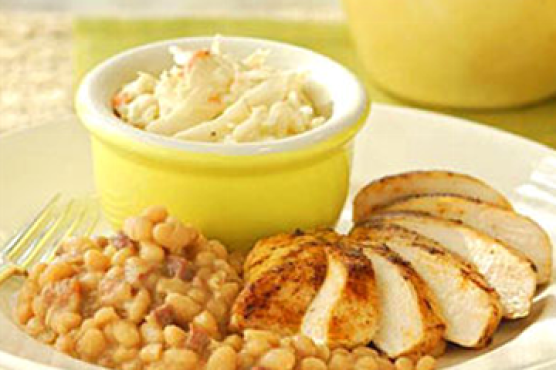
\includegraphics[width=\linewidth]{images/evaluation-images/baked_beans/baked-beans116.png}
\end{minipage}
\hfill
\begin{minipage}[t]{0.5\textwidth}
	\vspace{0pt}\raggedright
	\begin{tabularx}{\textwidth}{X r}
		\small \textbf{Real class} & \small Baked Beans\\
		\small \textbf{Predicted class} & \small Kebabs\\
		\small \textbf{Predicted accuracy} & \small 71.26 \%
    \end{tabularx}\\
    
    \vspace{6pt}
	\begin{tabularx}{\textwidth}{X r}
        \small \textbf{Top-5} & \small \textbf{Accuracy} \\
        \hline
		\small 1) Kebabs & \small 71.26 \%\\\small 2) Popcorn & \small 7.35 \%\\\small 3) Macaroni And Cheese & \small 3.03 \%\\\small 4) Key Lime Pie & \small 2.59 \%\\\small 5) Ice Cream & \small 2.55 \%
    \end{tabularx}
\end{minipage}
    
\subsection{Baked Salmon}
    
\subsubsection{baked\textunderscore salmon/baked-salmon11.jpg}

\begin{minipage}[t]{0.4\textwidth}
	\vspace{0pt}
	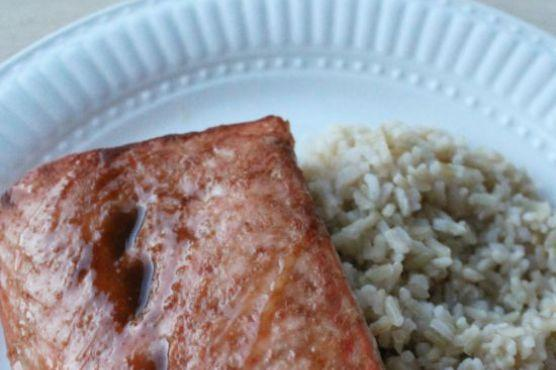
\includegraphics[width=\linewidth]{images/evaluation-images/baked_salmon/baked-salmon11.jpg}
\end{minipage}
\hfill
\begin{minipage}[t]{0.5\textwidth}
	\vspace{0pt}\raggedright
	\begin{tabularx}{\textwidth}{X r}
		\small \textbf{Real class} & \small Baked Salmon\\
		\small \textbf{Predicted class} & \small Empanada\\
		\small \textbf{Predicted accuracy} & \small 94.33 \%
    \end{tabularx}\\
    
    \vspace{6pt}
	\begin{tabularx}{\textwidth}{X r}
        \small \textbf{Top-5} & \small \textbf{Accuracy} \\
        \hline
		\small 1) Empanada & \small 94.33 \%\\\small 2) Omelet & \small 1.27 \%\\\small 3) Buttermilk Biscuits & \small 1.04 \%\\\small 4) Calzone & \small 0.94 \%\\\small 5) Cheesecake & \small 0.75 \%
    \end{tabularx}
\end{minipage}
    
\subsubsection{baked\textunderscore salmon/baked-salmon36.jpg}

\begin{minipage}[t]{0.4\textwidth}
	\vspace{0pt}
	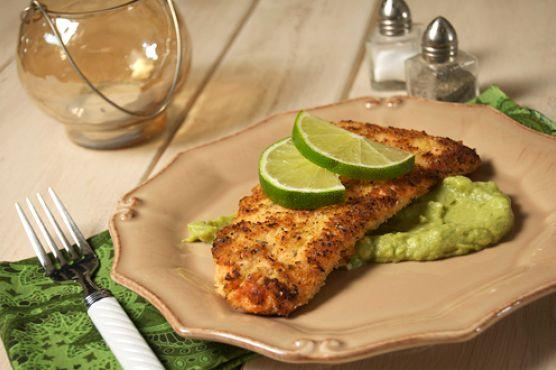
\includegraphics[width=\linewidth]{images/evaluation-images/baked_salmon/baked-salmon36.jpg}
\end{minipage}
\hfill
\begin{minipage}[t]{0.5\textwidth}
	\vspace{0pt}\raggedright
	\begin{tabularx}{\textwidth}{X r}
		\small \textbf{Real class} & \small Baked Salmon\\
		\small \textbf{Predicted class} & \small Caesar Salad\\
		\small \textbf{Predicted accuracy} & \small 45.25 \%
    \end{tabularx}\\
    
    \vspace{6pt}
	\begin{tabularx}{\textwidth}{X r}
        \small \textbf{Top-5} & \small \textbf{Accuracy} \\
        \hline
		\small 1) Caesar Salad & \small 45.25 \%\\\small 2) Frittata & \small 34.96 \%\\\small 3) Chicken Piccata & \small 7.58 \%\\\small 4) Grilled Cheese Sandwich & \small 3.79 \%\\\small 5) Key Lime Pie & \small 1.86 \%
    \end{tabularx}
\end{minipage}
    
\subsubsection{baked\textunderscore salmon/baked-salmon60.png}

\begin{minipage}[t]{0.4\textwidth}
	\vspace{0pt}
	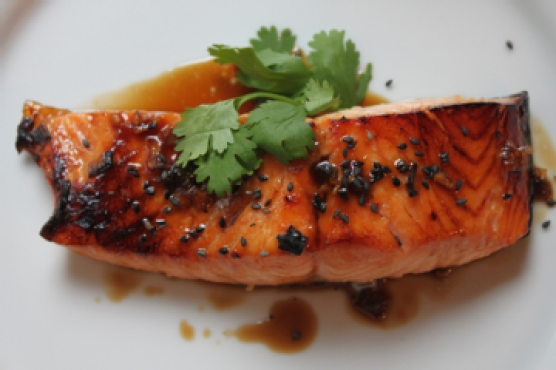
\includegraphics[width=\linewidth]{images/evaluation-images/baked_salmon/baked-salmon60.png}
\end{minipage}
\hfill
\begin{minipage}[t]{0.5\textwidth}
	\vspace{0pt}\raggedright
	\begin{tabularx}{\textwidth}{X r}
		\small \textbf{Real class} & \small Baked Salmon\\
		\small \textbf{Predicted class} & \small Chicken Piccata\\
		\small \textbf{Predicted accuracy} & \small 99.98 \%
    \end{tabularx}\\
    
    \vspace{6pt}
	\begin{tabularx}{\textwidth}{X r}
        \small \textbf{Top-5} & \small \textbf{Accuracy} \\
        \hline
		\small 1) Chicken Piccata & \small 99.98 \%\\\small 2) Stuffed Pepper & \small 0.01 \%\\\small 3) Chicken Wings & \small 0.00 \%\\\small 4) Quesadilla & \small 0.00 \%\\\small 5) Kebabs & \small 0.00 \%
    \end{tabularx}
\end{minipage}
    
\subsubsection{baked\textunderscore salmon/baked-salmon8.jpg}

\begin{minipage}[t]{0.4\textwidth}
	\vspace{0pt}
	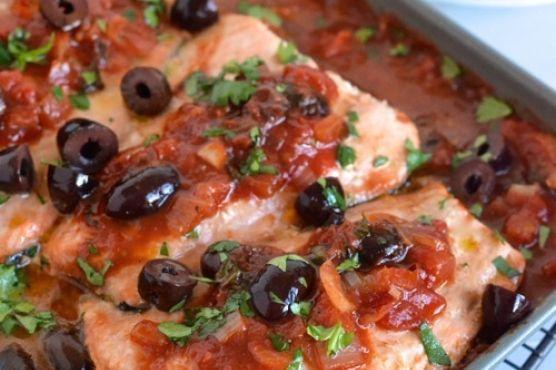
\includegraphics[width=\linewidth]{images/evaluation-images/baked_salmon/baked-salmon8.jpg}
\end{minipage}
\hfill
\begin{minipage}[t]{0.5\textwidth}
	\vspace{0pt}\raggedright
	\begin{tabularx}{\textwidth}{X r}
		\small \textbf{Real class} & \small Baked Salmon\\
		\small \textbf{Predicted class} & \small Nachos\\
		\small \textbf{Predicted accuracy} & \small 65.11 \%
    \end{tabularx}\\
    
    \vspace{6pt}
	\begin{tabularx}{\textwidth}{X r}
        \small \textbf{Top-5} & \small \textbf{Accuracy} \\
        \hline
		\small 1) Nachos & \small 65.11 \%\\\small 2) Chicken Piccata & \small 32.72 \%\\\small 3) Pizza & \small 2.01 \%\\\small 4) Meatballs & \small 0.05 \%\\\small 5) Soup & \small 0.04 \%
    \end{tabularx}
\end{minipage}
    
\subsection{Beef Stew}
    
\subsubsection{beef\textunderscore stew/beef-stew177.jpg}

\begin{minipage}[t]{0.4\textwidth}
	\vspace{0pt}
	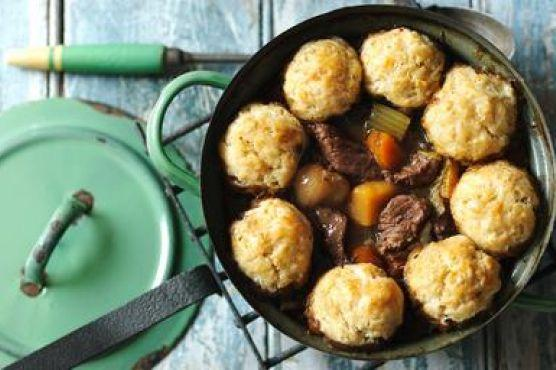
\includegraphics[width=\linewidth]{images/evaluation-images/beef_stew/beef-stew177.jpg}
\end{minipage}
\hfill
\begin{minipage}[t]{0.5\textwidth}
	\vspace{0pt}\raggedright
	\begin{tabularx}{\textwidth}{X r}
		\small \textbf{Real class} & \small Beef Stew\\
		\small \textbf{Predicted class} & \small Muffin\\
		\small \textbf{Predicted accuracy} & \small 100.00 \%
    \end{tabularx}\\
    
    \vspace{6pt}
	\begin{tabularx}{\textwidth}{X r}
        \small \textbf{Top-5} & \small \textbf{Accuracy} \\
        \hline
		\small 1) Muffin & \small 100.00 \%\\\small 2) Frittata & \small 0.00 \%\\\small 3) Meatballs & \small 0.00 \%\\\small 4) Kebabs & \small 0.00 \%\\\small 5) Brownies & \small 0.00 \%
    \end{tabularx}
\end{minipage}
    
\subsubsection{beef\textunderscore stew/beef-stew236.jpg}

\begin{minipage}[t]{0.4\textwidth}
	\vspace{0pt}
	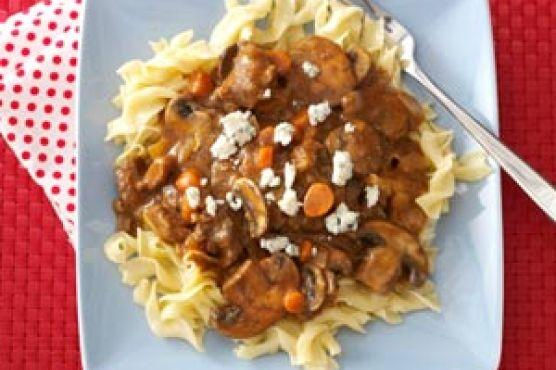
\includegraphics[width=\linewidth]{images/evaluation-images/beef_stew/beef-stew236.jpg}
\end{minipage}
\hfill
\begin{minipage}[t]{0.5\textwidth}
	\vspace{0pt}\raggedright
	\begin{tabularx}{\textwidth}{X r}
		\small \textbf{Real class} & \small Beef Stew\\
		\small \textbf{Predicted class} & \small Meatballs\\
		\small \textbf{Predicted accuracy} & \small 89.12 \%
    \end{tabularx}\\
    
    \vspace{6pt}
	\begin{tabularx}{\textwidth}{X r}
        \small \textbf{Top-5} & \small \textbf{Accuracy} \\
        \hline
		\small 1) Meatballs & \small 89.12 \%\\\small 2) Spaghetti & \small 3.95 \%\\\small 3) Popcorn & \small 2.70 \%\\\small 4) Beef Stroganoff & \small 1.53 \%\\\small 5) Nachos & \small 1.07 \%
    \end{tabularx}
\end{minipage}
    
\subsubsection{beef\textunderscore stew/beef-stew288.jpg}

\begin{minipage}[t]{0.4\textwidth}
	\vspace{0pt}
	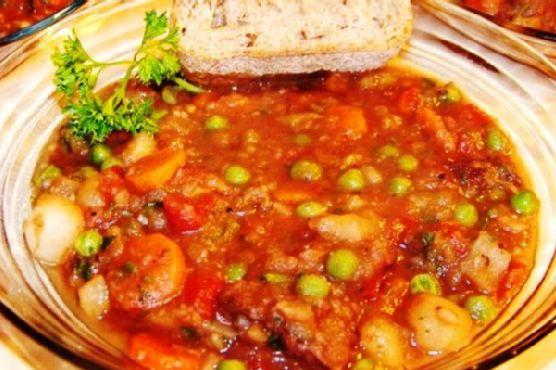
\includegraphics[width=\linewidth]{images/evaluation-images/beef_stew/beef-stew288.jpg}
\end{minipage}
\hfill
\begin{minipage}[t]{0.5\textwidth}
	\vspace{0pt}\raggedright
	\begin{tabularx}{\textwidth}{X r}
		\small \textbf{Real class} & \small Beef Stew\\
		\small \textbf{Predicted class} & \small Soup\\
		\small \textbf{Predicted accuracy} & \small 73.90 \%
    \end{tabularx}\\
    
    \vspace{6pt}
	\begin{tabularx}{\textwidth}{X r}
        \small \textbf{Top-5} & \small \textbf{Accuracy} \\
        \hline
		\small 1) Soup & \small 73.90 \%\\\small 2) Baked Beans & \small 20.75 \%\\\small 3) Meatballs & \small 2.33 \%\\\small 4) Spaghetti & \small 1.59 \%\\\small 5) Sloppy Joe & \small 0.71 \%
    \end{tabularx}
\end{minipage}
    
\subsubsection{beef\textunderscore stew/beef-stew33.jpg}

\begin{minipage}[t]{0.4\textwidth}
	\vspace{0pt}
	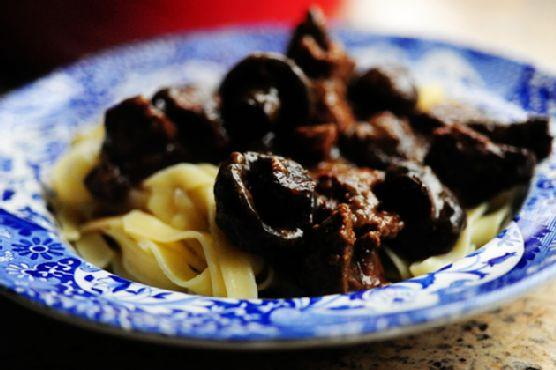
\includegraphics[width=\linewidth]{images/evaluation-images/beef_stew/beef-stew33.jpg}
\end{minipage}
\hfill
\begin{minipage}[t]{0.5\textwidth}
	\vspace{0pt}\raggedright
	\begin{tabularx}{\textwidth}{X r}
		\small \textbf{Real class} & \small Beef Stew\\
		\small \textbf{Predicted class} & \small Brownies\\
		\small \textbf{Predicted accuracy} & \small 98.63 \%
    \end{tabularx}\\
    
    \vspace{6pt}
	\begin{tabularx}{\textwidth}{X r}
        \small \textbf{Top-5} & \small \textbf{Accuracy} \\
        \hline
		\small 1) Brownies & \small 98.63 \%\\\small 2) Bundt Cake & \small 0.60 \%\\\small 3) Creamed Spinach & \small 0.21 \%\\\small 4) Margarita & \small 0.07 \%\\\small 5) Cheesecake & \small 0.07 \%
    \end{tabularx}
\end{minipage}
    
\subsection{Beef Stroganoff}
    
\subsubsection{beef\textunderscore stroganoff/beef-stroganoff122.jpg}

\begin{minipage}[t]{0.4\textwidth}
	\vspace{0pt}
	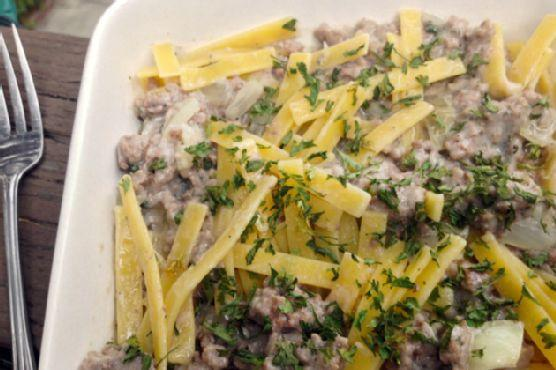
\includegraphics[width=\linewidth]{images/evaluation-images/beef_stroganoff/beef-stroganoff122.jpg}
\end{minipage}
\hfill
\begin{minipage}[t]{0.5\textwidth}
	\vspace{0pt}\raggedright
	\begin{tabularx}{\textwidth}{X r}
		\small \textbf{Real class} & \small Beef Stroganoff\\
		\small \textbf{Predicted class} & \small Salad\\
		\small \textbf{Predicted accuracy} & \small 68.95 \%
    \end{tabularx}\\
    
    \vspace{6pt}
	\begin{tabularx}{\textwidth}{X r}
        \small \textbf{Top-5} & \small \textbf{Accuracy} \\
        \hline
		\small 1) Salad & \small 68.95 \%\\\small 2) Nachos & \small 9.25 \%\\\small 3) Guacamole & \small 7.05 \%\\\small 4) Macaroni And Cheese & \small 3.53 \%\\\small 5) Omelet & \small 2.20 \%
    \end{tabularx}
\end{minipage}
    
\subsection{Brownies}
    
\subsubsection{brownies/brownies224.jpg}

\begin{minipage}[t]{0.4\textwidth}
	\vspace{0pt}
	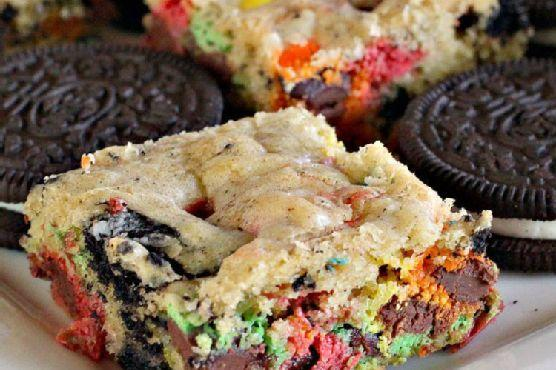
\includegraphics[width=\linewidth]{images/evaluation-images/brownies/brownies224.jpg}
\end{minipage}
\hfill
\begin{minipage}[t]{0.5\textwidth}
	\vspace{0pt}\raggedright
	\begin{tabularx}{\textwidth}{X r}
		\small \textbf{Real class} & \small Brownies\\
		\small \textbf{Predicted class} & \small Frittata\\
		\small \textbf{Predicted accuracy} & \small 66.18 \%
    \end{tabularx}\\
    
    \vspace{6pt}
	\begin{tabularx}{\textwidth}{X r}
        \small \textbf{Top-5} & \small \textbf{Accuracy} \\
        \hline
		\small 1) Frittata & \small 66.18 \%\\\small 2) Pizza & \small 11.16 \%\\\small 3) Meatloaf & \small 6.02 \%\\\small 4) Cinnamon Roll & \small 4.60 \%\\\small 5) Muffin & \small 4.39 \%
    \end{tabularx}
\end{minipage}
    
\subsection{Burger}
    
\subsubsection{burger/burger30.jpg}

\begin{minipage}[t]{0.4\textwidth}
	\vspace{0pt}
	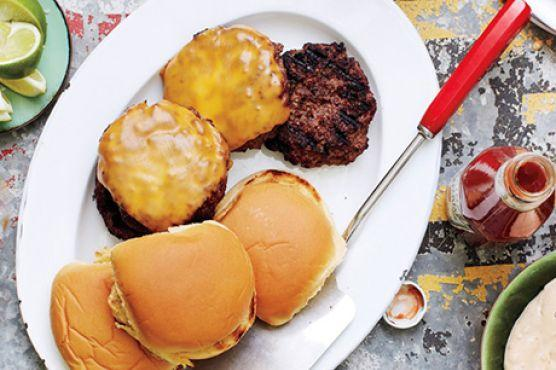
\includegraphics[width=\linewidth]{images/evaluation-images/burger/burger30.jpg}
\end{minipage}
\hfill
\begin{minipage}[t]{0.5\textwidth}
	\vspace{0pt}\raggedright
	\begin{tabularx}{\textwidth}{X r}
		\small \textbf{Real class} & \small Burger\\
		\small \textbf{Predicted class} & \small Meatballs\\
		\small \textbf{Predicted accuracy} & \small 65.13 \%
    \end{tabularx}\\
    
    \vspace{6pt}
	\begin{tabularx}{\textwidth}{X r}
        \small \textbf{Top-5} & \small \textbf{Accuracy} \\
        \hline
		\small 1) Meatballs & \small 65.13 \%\\\small 2) Muffin & \small 9.94 \%\\\small 3) Stuffed Pepper & \small 9.71 \%\\\small 4) Ice Cream & \small 5.97 \%\\\small 5) Kebabs & \small 2.62 \%
    \end{tabularx}
\end{minipage}
    
\subsection{Burrito}
    
\subsubsection{burrito/burrito99.jpg}

\begin{minipage}[t]{0.4\textwidth}
	\vspace{0pt}
	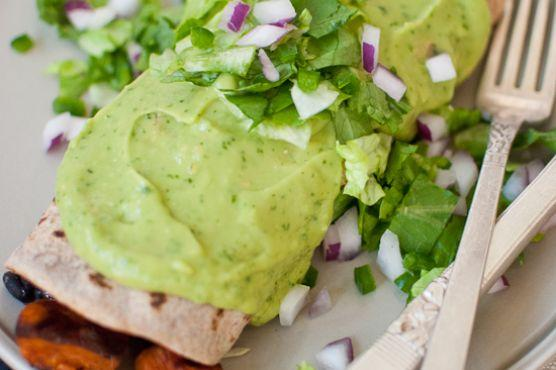
\includegraphics[width=\linewidth]{images/evaluation-images/burrito/burrito99.jpg}
\end{minipage}
\hfill
\begin{minipage}[t]{0.5\textwidth}
	\vspace{0pt}\raggedright
	\begin{tabularx}{\textwidth}{X r}
		\small \textbf{Real class} & \small Burrito\\
		\small \textbf{Predicted class} & \small Omelet\\
		\small \textbf{Predicted accuracy} & \small 47.12 \%
    \end{tabularx}\\
    
    \vspace{6pt}
	\begin{tabularx}{\textwidth}{X r}
        \small \textbf{Top-5} & \small \textbf{Accuracy} \\
        \hline
		\small 1) Omelet & \small 47.12 \%\\\small 2) Guacamole & \small 42.63 \%\\\small 3) Salad & \small 8.77 \%\\\small 4) Sloppy Joe & \small 0.66 \%\\\small 5) Cobb Salad & \small 0.22 \%
    \end{tabularx}
\end{minipage}
    
\subsection{Calzone}
    
\subsubsection{calzone/calzone166.jpg}

\begin{minipage}[t]{0.4\textwidth}
	\vspace{0pt}
	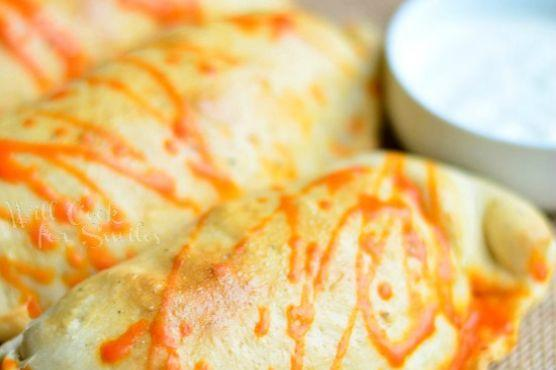
\includegraphics[width=\linewidth]{images/evaluation-images/calzone/calzone166.jpg}
\end{minipage}
\hfill
\begin{minipage}[t]{0.5\textwidth}
	\vspace{0pt}\raggedright
	\begin{tabularx}{\textwidth}{X r}
		\small \textbf{Real class} & \small Calzone\\
		\small \textbf{Predicted class} & \small Baked Salmon\\
		\small \textbf{Predicted accuracy} & \small 94.12 \%
    \end{tabularx}\\
    
    \vspace{6pt}
	\begin{tabularx}{\textwidth}{X r}
        \small \textbf{Top-5} & \small \textbf{Accuracy} \\
        \hline
		\small 1) Baked Salmon & \small 94.12 \%\\\small 2) Empanada & \small 1.65 \%\\\small 3) Chicken Piccata & \small 1.53 \%\\\small 4) Quesadilla & \small 0.86 \%\\\small 5) Smoothie & \small 0.42 \%
    \end{tabularx}
\end{minipage}
    
\subsubsection{calzone/calzone52.jpg}

\begin{minipage}[t]{0.4\textwidth}
	\vspace{0pt}
	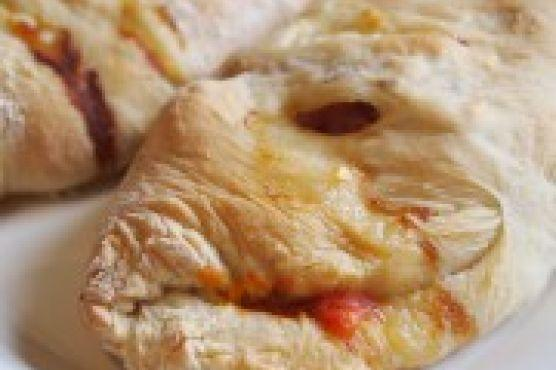
\includegraphics[width=\linewidth]{images/evaluation-images/calzone/calzone52.jpg}
\end{minipage}
\hfill
\begin{minipage}[t]{0.5\textwidth}
	\vspace{0pt}\raggedright
	\begin{tabularx}{\textwidth}{X r}
		\small \textbf{Real class} & \small Calzone\\
		\small \textbf{Predicted class} & \small Pizza\\
		\small \textbf{Predicted accuracy} & \small 54.22 \%
    \end{tabularx}\\
    
    \vspace{6pt}
	\begin{tabularx}{\textwidth}{X r}
        \small \textbf{Top-5} & \small \textbf{Accuracy} \\
        \hline
		\small 1) Pizza & \small 54.22 \%\\\small 2) Cinnamon Roll & \small 24.46 \%\\\small 3) Baked Salmon & \small 13.00 \%\\\small 4) Donut & \small 5.38 \%\\\small 5) Burrito & \small 1.61 \%
    \end{tabularx}
\end{minipage}
    
\subsection{Cheesecake}
    
\subsubsection{cheesecake/cheesecake45.jpg}

\begin{minipage}[t]{0.4\textwidth}
	\vspace{0pt}
	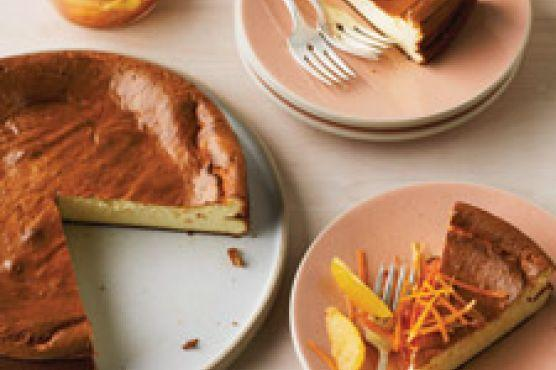
\includegraphics[width=\linewidth]{images/evaluation-images/cheesecake/cheesecake45.jpg}
\end{minipage}
\hfill
\begin{minipage}[t]{0.5\textwidth}
	\vspace{0pt}\raggedright
	\begin{tabularx}{\textwidth}{X r}
		\small \textbf{Real class} & \small Cheesecake\\
		\small \textbf{Predicted class} & \small Calzone\\
		\small \textbf{Predicted accuracy} & \small 100.00 \%
    \end{tabularx}\\
    
    \vspace{6pt}
	\begin{tabularx}{\textwidth}{X r}
        \small \textbf{Top-5} & \small \textbf{Accuracy} \\
        \hline
		\small 1) Calzone & \small 100.00 \%\\\small 2) Empanada & \small 0.00 \%\\\small 3) Pizza & \small 0.00 \%\\\small 4) Burrito & \small 0.00 \%\\\small 5) Omelet & \small 0.00 \%
    \end{tabularx}
\end{minipage}
    
\subsubsection{cheesecake/cheesecake469.jpg}

\begin{minipage}[t]{0.4\textwidth}
	\vspace{0pt}
	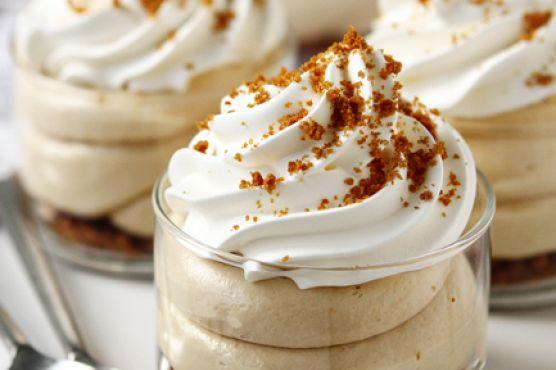
\includegraphics[width=\linewidth]{images/evaluation-images/cheesecake/cheesecake469.jpg}
\end{minipage}
\hfill
\begin{minipage}[t]{0.5\textwidth}
	\vspace{0pt}\raggedright
	\begin{tabularx}{\textwidth}{X r}
		\small \textbf{Real class} & \small Cheesecake\\
		\small \textbf{Predicted class} & \small Cinnamon Roll\\
		\small \textbf{Predicted accuracy} & \small 100.00 \%
    \end{tabularx}\\
    
    \vspace{6pt}
	\begin{tabularx}{\textwidth}{X r}
        \small \textbf{Top-5} & \small \textbf{Accuracy} \\
        \hline
		\small 1) Cinnamon Roll & \small 100.00 \%\\\small 2) Key Lime Pie & \small 0.00 \%\\\small 3) Donut & \small 0.00 \%\\\small 4) Mashed Potatoes & \small 0.00 \%\\\small 5) Ice Cream & \small 0.00 \%
    \end{tabularx}
\end{minipage}
    
\subsection{Chicken Piccata}
    
\subsubsection{chicken\textunderscore piccata/chicken-piccata38.jpg}

\begin{minipage}[t]{0.4\textwidth}
	\vspace{0pt}
	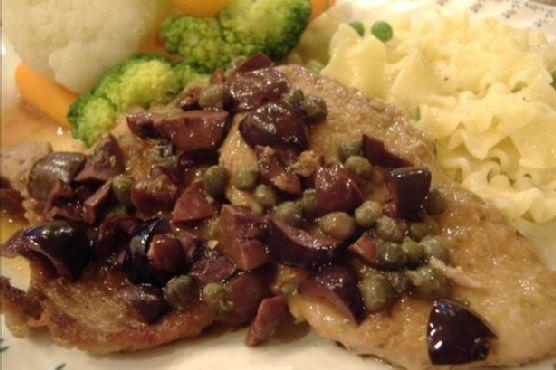
\includegraphics[width=\linewidth]{images/evaluation-images/chicken_piccata/chicken-piccata38.jpg}
\end{minipage}
\hfill
\begin{minipage}[t]{0.5\textwidth}
	\vspace{0pt}\raggedright
	\begin{tabularx}{\textwidth}{X r}
		\small \textbf{Real class} & \small Chicken Piccata\\
		\small \textbf{Predicted class} & \small Beef Stew\\
		\small \textbf{Predicted accuracy} & \small 65.51 \%
    \end{tabularx}\\
    
    \vspace{6pt}
	\begin{tabularx}{\textwidth}{X r}
        \small \textbf{Top-5} & \small \textbf{Accuracy} \\
        \hline
		\small 1) Beef Stew & \small 65.51 \%\\\small 2) Beef Stroganoff & \small 23.25 \%\\\small 3) Meatloaf & \small 5.18 \%\\\small 4) Sloppy Joe & \small 2.56 \%\\\small 5) Meatballs & \small 1.98 \%
    \end{tabularx}
\end{minipage}
    
\subsection{Cinnamon Roll}
    
\subsubsection{cinnamon\textunderscore roll/cinnamon-roll384.jpg}

\begin{minipage}[t]{0.4\textwidth}
	\vspace{0pt}
	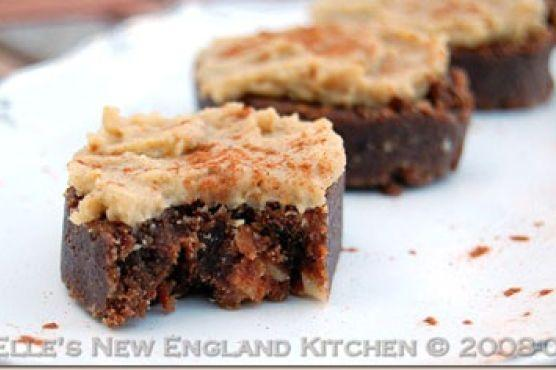
\includegraphics[width=\linewidth]{images/evaluation-images/cinnamon_roll/cinnamon-roll384.jpg}
\end{minipage}
\hfill
\begin{minipage}[t]{0.5\textwidth}
	\vspace{0pt}\raggedright
	\begin{tabularx}{\textwidth}{X r}
		\small \textbf{Real class} & \small Cinnamon Roll\\
		\small \textbf{Predicted class} & \small Brownies\\
		\small \textbf{Predicted accuracy} & \small 99.92 \%
    \end{tabularx}\\
    
    \vspace{6pt}
	\begin{tabularx}{\textwidth}{X r}
        \small \textbf{Top-5} & \small \textbf{Accuracy} \\
        \hline
		\small 1) Brownies & \small 99.92 \%\\\small 2) Muffin & \small 0.06 \%\\\small 3) Cheesecake & \small 0.01 \%\\\small 4) Granola Bar & \small 0.00 \%\\\small 5) Meatloaf & \small 0.00 \%
    \end{tabularx}
\end{minipage}
    
\subsection{Corn Dog}
    
\subsubsection{corn\textunderscore dog/corn-dog25.jpg}

\begin{minipage}[t]{0.4\textwidth}
	\vspace{0pt}
	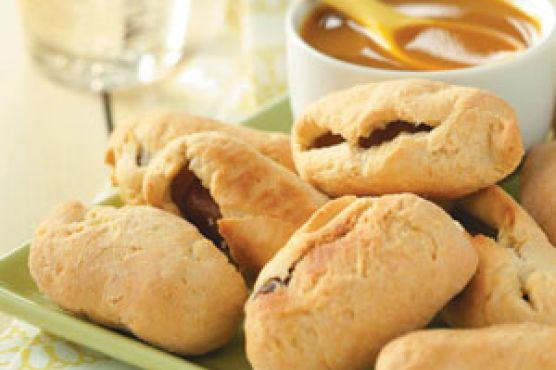
\includegraphics[width=\linewidth]{images/evaluation-images/corn_dog/corn-dog25.jpg}
\end{minipage}
\hfill
\begin{minipage}[t]{0.5\textwidth}
	\vspace{0pt}\raggedright
	\begin{tabularx}{\textwidth}{X r}
		\small \textbf{Real class} & \small Corn Dog\\
		\small \textbf{Predicted class} & \small Empanada\\
		\small \textbf{Predicted accuracy} & \small 100.00 \%
    \end{tabularx}\\
    
    \vspace{6pt}
	\begin{tabularx}{\textwidth}{X r}
        \small \textbf{Top-5} & \small \textbf{Accuracy} \\
        \hline
		\small 1) Empanada & \small 100.00 \%\\\small 2) Donut & \small 0.00 \%\\\small 3) Buttermilk Biscuits & \small 0.00 \%\\\small 4) Chicken Wings & \small 0.00 \%\\\small 5) Calzone & \small 0.00 \%
    \end{tabularx}
\end{minipage}
    
\subsubsection{corn\textunderscore dog/corn-dog26.jpg}

\begin{minipage}[t]{0.4\textwidth}
	\vspace{0pt}
	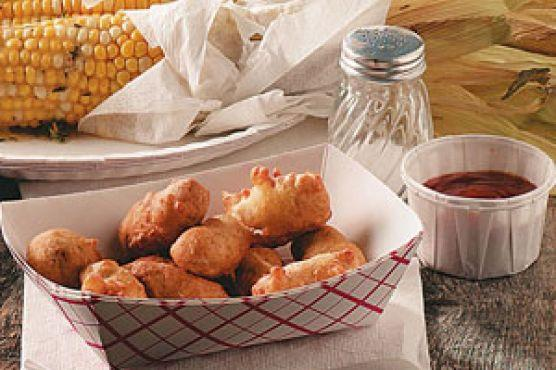
\includegraphics[width=\linewidth]{images/evaluation-images/corn_dog/corn-dog26.jpg}
\end{minipage}
\hfill
\begin{minipage}[t]{0.5\textwidth}
	\vspace{0pt}\raggedright
	\begin{tabularx}{\textwidth}{X r}
		\small \textbf{Real class} & \small Corn Dog\\
		\small \textbf{Predicted class} & \small Meatballs\\
		\small \textbf{Predicted accuracy} & \small 55.30 \%
    \end{tabularx}\\
    
    \vspace{6pt}
	\begin{tabularx}{\textwidth}{X r}
        \small \textbf{Top-5} & \small \textbf{Accuracy} \\
        \hline
		\small 1) Meatballs & \small 55.30 \%\\\small 2) Buttermilk Biscuits & \small 15.89 \%\\\small 3) Muffin & \small 15.69 \%\\\small 4) Empanada & \small 6.31 \%\\\small 5) Chicken Wings & \small 1.10 \%
    \end{tabularx}
\end{minipage}
    
\subsection{Donut}
    
\subsubsection{donut/donut286.jpg}

\begin{minipage}[t]{0.4\textwidth}
	\vspace{0pt}
	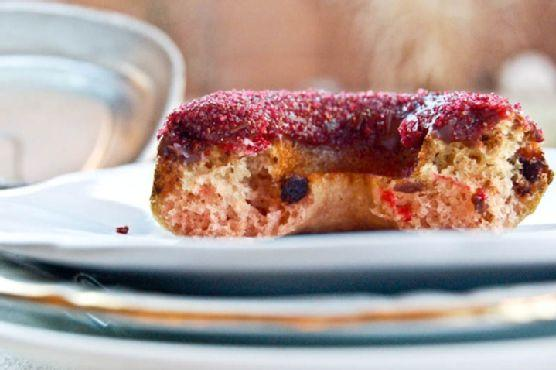
\includegraphics[width=\linewidth]{images/evaluation-images/donut/donut286.jpg}
\end{minipage}
\hfill
\begin{minipage}[t]{0.5\textwidth}
	\vspace{0pt}\raggedright
	\begin{tabularx}{\textwidth}{X r}
		\small \textbf{Real class} & \small Donut\\
		\small \textbf{Predicted class} & \small Muffin\\
		\small \textbf{Predicted accuracy} & \small 93.54 \%
    \end{tabularx}\\
    
    \vspace{6pt}
	\begin{tabularx}{\textwidth}{X r}
        \small \textbf{Top-5} & \small \textbf{Accuracy} \\
        \hline
		\small 1) Muffin & \small 93.54 \%\\\small 2) Bundt Cake & \small 2.58 \%\\\small 3) Meatloaf & \small 1.83 \%\\\small 4) Granola Bar & \small 1.04 \%\\\small 5) Grilled Cheese Sandwich & \small 0.45 \%
    \end{tabularx}
\end{minipage}
    
\subsubsection{donut/donut408.jpg}

\begin{minipage}[t]{0.4\textwidth}
	\vspace{0pt}
	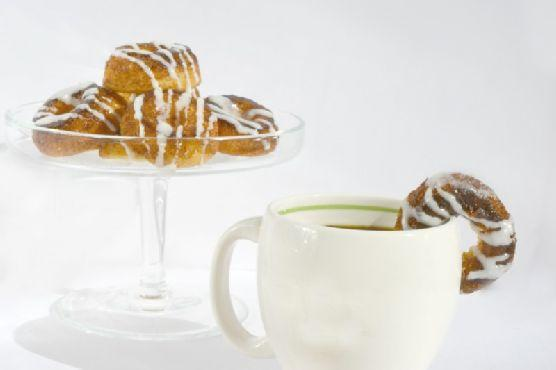
\includegraphics[width=\linewidth]{images/evaluation-images/donut/donut408.jpg}
\end{minipage}
\hfill
\begin{minipage}[t]{0.5\textwidth}
	\vspace{0pt}\raggedright
	\begin{tabularx}{\textwidth}{X r}
		\small \textbf{Real class} & \small Donut\\
		\small \textbf{Predicted class} & \small Margarita\\
		\small \textbf{Predicted accuracy} & \small 96.76 \%
    \end{tabularx}\\
    
    \vspace{6pt}
	\begin{tabularx}{\textwidth}{X r}
        \small \textbf{Top-5} & \small \textbf{Accuracy} \\
        \hline
		\small 1) Margarita & \small 96.76 \%\\\small 2) Smoothie & \small 3.00 \%\\\small 3) Martini & \small 0.10 \%\\\small 4) Spaghetti & \small 0.02 \%\\\small 5) Bundt Cake & \small 0.01 \%
    \end{tabularx}
\end{minipage}
    
\subsection{Empanada}
    
\subsubsection{empanada/empanada118.jpg}

\begin{minipage}[t]{0.4\textwidth}
	\vspace{0pt}
	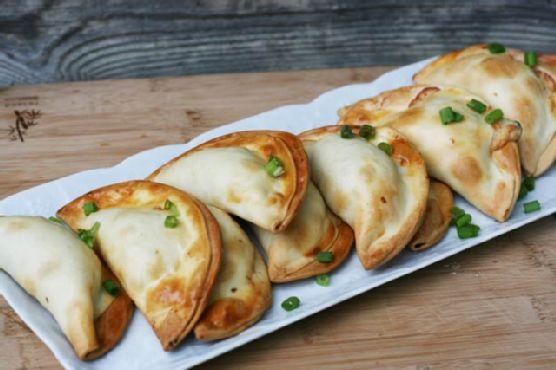
\includegraphics[width=\linewidth]{images/evaluation-images/empanada/empanada118.jpg}
\end{minipage}
\hfill
\begin{minipage}[t]{0.5\textwidth}
	\vspace{0pt}\raggedright
	\begin{tabularx}{\textwidth}{X r}
		\small \textbf{Real class} & \small Empanada\\
		\small \textbf{Predicted class} & \small Quesadilla\\
		\small \textbf{Predicted accuracy} & \small 51.52 \%
    \end{tabularx}\\
    
    \vspace{6pt}
	\begin{tabularx}{\textwidth}{X r}
        \small \textbf{Top-5} & \small \textbf{Accuracy} \\
        \hline
		\small 1) Quesadilla & \small 51.52 \%\\\small 2) Calzone & \small 45.49 \%\\\small 3) Burrito & \small 1.33 \%\\\small 4) Pizza & \small 0.70 \%\\\small 5) Cinnamon Roll & \small 0.42 \%
    \end{tabularx}
\end{minipage}
    
\subsubsection{empanada/empanada34.jpg}

\begin{minipage}[t]{0.4\textwidth}
	\vspace{0pt}
	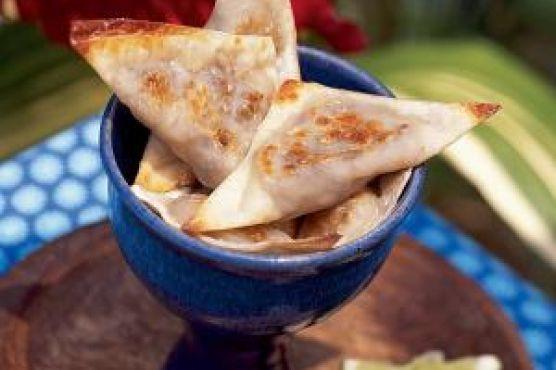
\includegraphics[width=\linewidth]{images/evaluation-images/empanada/empanada34.jpg}
\end{minipage}
\hfill
\begin{minipage}[t]{0.5\textwidth}
	\vspace{0pt}\raggedright
	\begin{tabularx}{\textwidth}{X r}
		\small \textbf{Real class} & \small Empanada\\
		\small \textbf{Predicted class} & \small Quesadilla\\
		\small \textbf{Predicted accuracy} & \small 99.90 \%
    \end{tabularx}\\
    
    \vspace{6pt}
	\begin{tabularx}{\textwidth}{X r}
        \small \textbf{Top-5} & \small \textbf{Accuracy} \\
        \hline
		\small 1) Quesadilla & \small 99.90 \%\\\small 2) Burrito & \small 0.03 \%\\\small 3) Margarita & \small 0.02 \%\\\small 4) Martini & \small 0.01 \%\\\small 5) Smoothie & \small 0.01 \%
    \end{tabularx}
\end{minipage}
    
\subsection{French Fries}
    
\subsubsection{french\textunderscore fries/french-fries19.jpg}

\begin{minipage}[t]{0.4\textwidth}
	\vspace{0pt}
	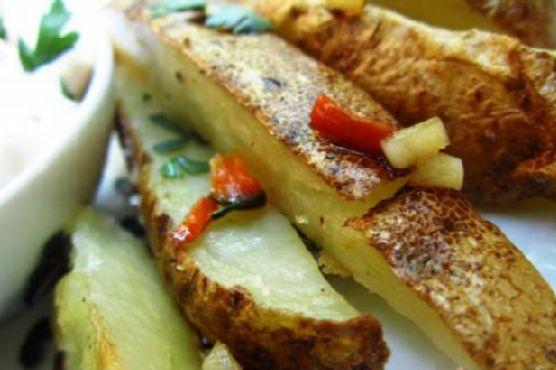
\includegraphics[width=\linewidth]{images/evaluation-images/french_fries/french-fries19.jpg}
\end{minipage}
\hfill
\begin{minipage}[t]{0.5\textwidth}
	\vspace{0pt}\raggedright
	\begin{tabularx}{\textwidth}{X r}
		\small \textbf{Real class} & \small French Fries\\
		\small \textbf{Predicted class} & \small Grilled Cheese Sandwich\\
		\small \textbf{Predicted accuracy} & \small 99.86 \%
    \end{tabularx}\\
    
    \vspace{6pt}
	\begin{tabularx}{\textwidth}{X r}
        \small \textbf{Top-5} & \small \textbf{Accuracy} \\
        \hline
		\small 1) Grilled Cheese Sandwich & \small 99.86 \%\\\small 2) Kebabs & \small 0.04 \%\\\small 3) Burger & \small 0.03 \%\\\small 4) Meatloaf & \small 0.03 \%\\\small 5) Omelet & \small 0.01 \%
    \end{tabularx}
\end{minipage}
    
\subsubsection{french\textunderscore fries/french-fries65.jpg}

\begin{minipage}[t]{0.4\textwidth}
	\vspace{0pt}
	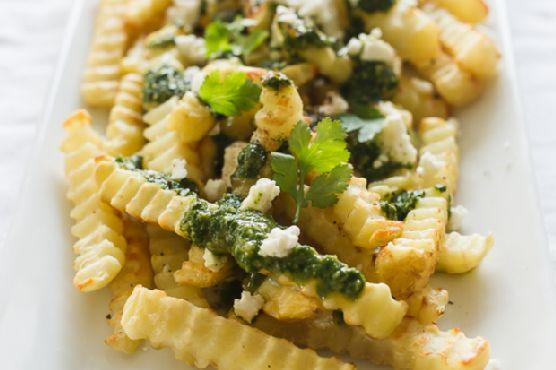
\includegraphics[width=\linewidth]{images/evaluation-images/french_fries/french-fries65.jpg}
\end{minipage}
\hfill
\begin{minipage}[t]{0.5\textwidth}
	\vspace{0pt}\raggedright
	\begin{tabularx}{\textwidth}{X r}
		\small \textbf{Real class} & \small French Fries\\
		\small \textbf{Predicted class} & \small Macaroni And Cheese\\
		\small \textbf{Predicted accuracy} & \small 40.54 \%
    \end{tabularx}\\
    
    \vspace{6pt}
	\begin{tabularx}{\textwidth}{X r}
        \small \textbf{Top-5} & \small \textbf{Accuracy} \\
        \hline
		\small 1) Macaroni And Cheese & \small 40.54 \%\\\small 2) Caesar Salad & \small 11.87 \%\\\small 3) Salad & \small 9.38 \%\\\small 4) Soup & \small 8.86 \%\\\small 5) Kebabs & \small 8.35 \%
    \end{tabularx}
\end{minipage}
    
\subsection{Frittata}
    
\subsubsection{frittata/frittata275.jpg}

\begin{minipage}[t]{0.4\textwidth}
	\vspace{0pt}
	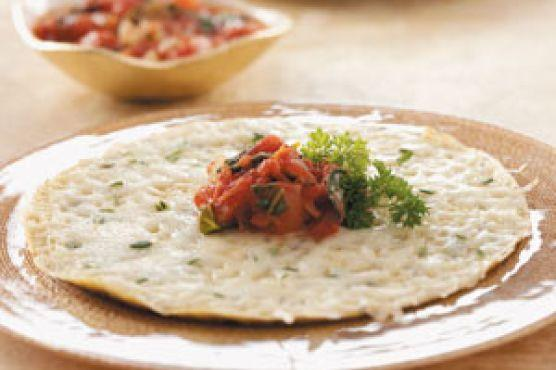
\includegraphics[width=\linewidth]{images/evaluation-images/frittata/frittata275.jpg}
\end{minipage}
\hfill
\begin{minipage}[t]{0.5\textwidth}
	\vspace{0pt}\raggedright
	\begin{tabularx}{\textwidth}{X r}
		\small \textbf{Real class} & \small Frittata\\
		\small \textbf{Predicted class} & \small Pancakes\\
		\small \textbf{Predicted accuracy} & \small 96.64 \%
    \end{tabularx}\\
    
    \vspace{6pt}
	\begin{tabularx}{\textwidth}{X r}
        \small \textbf{Top-5} & \small \textbf{Accuracy} \\
        \hline
		\small 1) Pancakes & \small 96.64 \%\\\small 2) Quesadilla & \small 3.30 \%\\\small 3) Omelet & \small 0.02 \%\\\small 4) Pizza & \small 0.01 \%\\\small 5) Waffles & \small 0.01 \%
    \end{tabularx}
\end{minipage}
    
\subsubsection{frittata/frittata283.jpg}

\begin{minipage}[t]{0.4\textwidth}
	\vspace{0pt}
	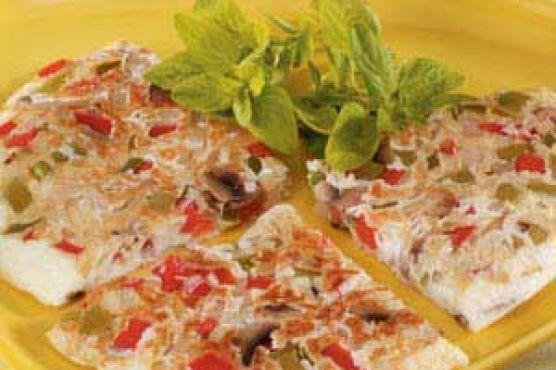
\includegraphics[width=\linewidth]{images/evaluation-images/frittata/frittata283.jpg}
\end{minipage}
\hfill
\begin{minipage}[t]{0.5\textwidth}
	\vspace{0pt}\raggedright
	\begin{tabularx}{\textwidth}{X r}
		\small \textbf{Real class} & \small Frittata\\
		\small \textbf{Predicted class} & \small Pizza\\
		\small \textbf{Predicted accuracy} & \small 99.82 \%
    \end{tabularx}\\
    
    \vspace{6pt}
	\begin{tabularx}{\textwidth}{X r}
        \small \textbf{Top-5} & \small \textbf{Accuracy} \\
        \hline
		\small 1) Pizza & \small 99.82 \%\\\small 2) Coleslaw & \small 0.12 \%\\\small 3) Nachos & \small 0.03 \%\\\small 4) Lasagne & \small 0.02 \%\\\small 5) Quesadilla & \small 0.00 \%
    \end{tabularx}
\end{minipage}
    
\subsubsection{frittata/frittata435.jpg}

\begin{minipage}[t]{0.4\textwidth}
	\vspace{0pt}
	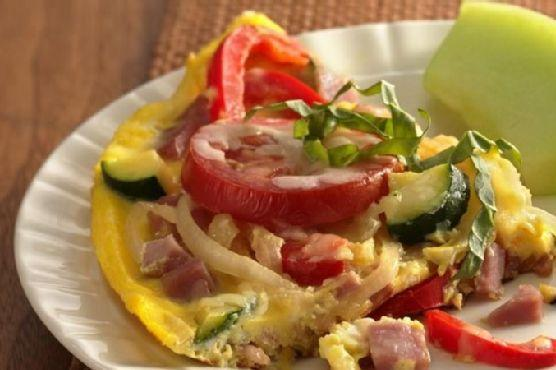
\includegraphics[width=\linewidth]{images/evaluation-images/frittata/frittata435.jpg}
\end{minipage}
\hfill
\begin{minipage}[t]{0.5\textwidth}
	\vspace{0pt}\raggedright
	\begin{tabularx}{\textwidth}{X r}
		\small \textbf{Real class} & \small Frittata\\
		\small \textbf{Predicted class} & \small Grilled Cheese Sandwich\\
		\small \textbf{Predicted accuracy} & \small 34.54 \%
    \end{tabularx}\\
    
    \vspace{6pt}
	\begin{tabularx}{\textwidth}{X r}
        \small \textbf{Top-5} & \small \textbf{Accuracy} \\
        \hline
		\small 1) Grilled Cheese Sandwich & \small 34.54 \%\\\small 2) Baked Salmon & \small 21.58 \%\\\small 3) Caesar Salad & \small 12.28 \%\\\small 4) Burger & \small 8.70 \%\\\small 5) Coleslaw & \small 6.60 \%
    \end{tabularx}
\end{minipage}
    
\subsection{Granola Bar}
    
\subsubsection{granola\textunderscore bar/granola-bar217.jpg}

\begin{minipage}[t]{0.4\textwidth}
	\vspace{0pt}
	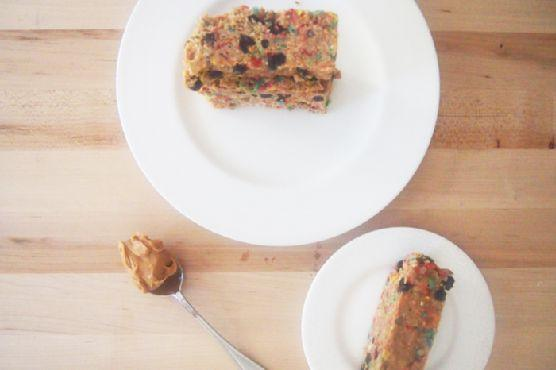
\includegraphics[width=\linewidth]{images/evaluation-images/granola_bar/granola-bar217.jpg}
\end{minipage}
\hfill
\begin{minipage}[t]{0.5\textwidth}
	\vspace{0pt}\raggedright
	\begin{tabularx}{\textwidth}{X r}
		\small \textbf{Real class} & \small Granola Bar\\
		\small \textbf{Predicted class} & \small Waffles\\
		\small \textbf{Predicted accuracy} & \small 97.12 \%
    \end{tabularx}\\
    
    \vspace{6pt}
	\begin{tabularx}{\textwidth}{X r}
        \small \textbf{Top-5} & \small \textbf{Accuracy} \\
        \hline
		\small 1) Waffles & \small 97.12 \%\\\small 2) Frittata & \small 0.92 \%\\\small 3) Cheesecake & \small 0.45 \%\\\small 4) Lasagne & \small 0.19 \%\\\small 5) Chicken Wings & \small 0.16 \%
    \end{tabularx}
\end{minipage}
    
\subsection{Grilled Cheese Sandwich}
    
\subsubsection{grilled\textunderscore cheese\textunderscore sandwich/grilled-cheese-sandwich109.jpg}

\begin{minipage}[t]{0.4\textwidth}
	\vspace{0pt}
	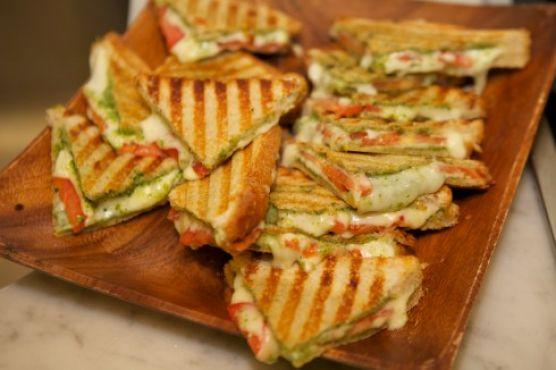
\includegraphics[width=\linewidth]{images/evaluation-images/grilled_cheese_sandwich/grilled-cheese-sandwich109.jpg}
\end{minipage}
\hfill
\begin{minipage}[t]{0.5\textwidth}
	\vspace{0pt}\raggedright
	\begin{tabularx}{\textwidth}{X r}
		\small \textbf{Real class} & \small Grilled Cheese Sandwich\\
		\small \textbf{Predicted class} & \small Calzone\\
		\small \textbf{Predicted accuracy} & \small 41.97 \%
    \end{tabularx}\\
    
    \vspace{6pt}
	\begin{tabularx}{\textwidth}{X r}
        \small \textbf{Top-5} & \small \textbf{Accuracy} \\
        \hline
		\small 1) Calzone & \small 41.97 \%\\\small 2) Omelet & \small 16.09 \%\\\small 3) Quesadilla & \small 6.74 \%\\\small 4) French Fries & \small 6.59 \%\\\small 5) Pancakes & \small 5.05 \%
    \end{tabularx}
\end{minipage}
    
\subsubsection{grilled\textunderscore cheese\textunderscore sandwich/grilled-cheese-sandwich221.jpg}

\begin{minipage}[t]{0.4\textwidth}
	\vspace{0pt}
	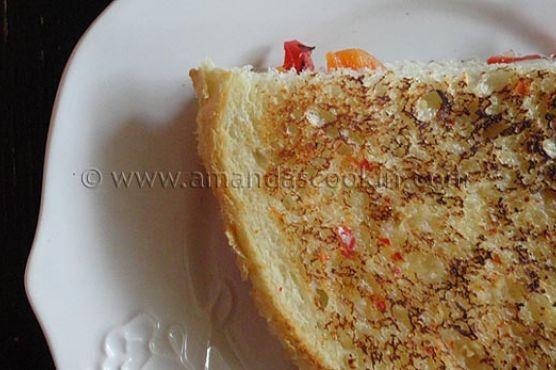
\includegraphics[width=\linewidth]{images/evaluation-images/grilled_cheese_sandwich/grilled-cheese-sandwich221.jpg}
\end{minipage}
\hfill
\begin{minipage}[t]{0.5\textwidth}
	\vspace{0pt}\raggedright
	\begin{tabularx}{\textwidth}{X r}
		\small \textbf{Real class} & \small Grilled Cheese Sandwich\\
		\small \textbf{Predicted class} & \small Cheesecake\\
		\small \textbf{Predicted accuracy} & \small 79.16 \%
    \end{tabularx}\\
    
    \vspace{6pt}
	\begin{tabularx}{\textwidth}{X r}
        \small \textbf{Top-5} & \small \textbf{Accuracy} \\
        \hline
		\small 1) Cheesecake & \small 79.16 \%\\\small 2) Bundt Cake & \small 9.78 \%\\\small 3) Omelet & \small 5.82 \%\\\small 4) Frittata & \small 4.77 \%\\\small 5) Key Lime Pie & \small 0.20 \%
    \end{tabularx}
\end{minipage}
    
\subsubsection{grilled\textunderscore cheese\textunderscore sandwich/grilled-cheese-sandwich448.jpg}

\begin{minipage}[t]{0.4\textwidth}
	\vspace{0pt}
	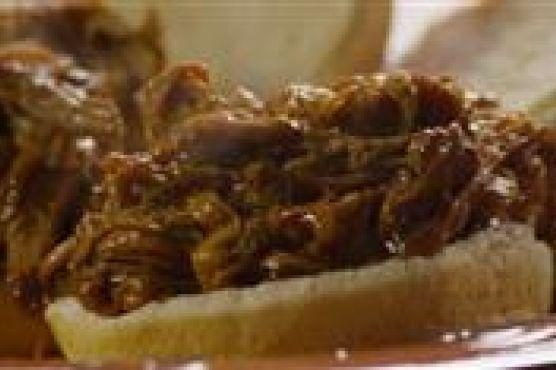
\includegraphics[width=\linewidth]{images/evaluation-images/grilled_cheese_sandwich/grilled-cheese-sandwich448.jpg}
\end{minipage}
\hfill
\begin{minipage}[t]{0.5\textwidth}
	\vspace{0pt}\raggedright
	\begin{tabularx}{\textwidth}{X r}
		\small \textbf{Real class} & \small Grilled Cheese Sandwich\\
		\small \textbf{Predicted class} & \small Sloppy Joe\\
		\small \textbf{Predicted accuracy} & \small 95.37 \%
    \end{tabularx}\\
    
    \vspace{6pt}
	\begin{tabularx}{\textwidth}{X r}
        \small \textbf{Top-5} & \small \textbf{Accuracy} \\
        \hline
		\small 1) Sloppy Joe & \small 95.37 \%\\\small 2) Pizza & \small 4.45 \%\\\small 3) Burger & \small 0.09 \%\\\small 4) Cheesecake & \small 0.03 \%\\\small 5) Chicken Wings & \small 0.01 \%
    \end{tabularx}
\end{minipage}
    
\subsubsection{grilled\textunderscore cheese\textunderscore sandwich/grilled-cheese-sandwich457.jpeg}

\begin{minipage}[t]{0.4\textwidth}
	\vspace{0pt}
	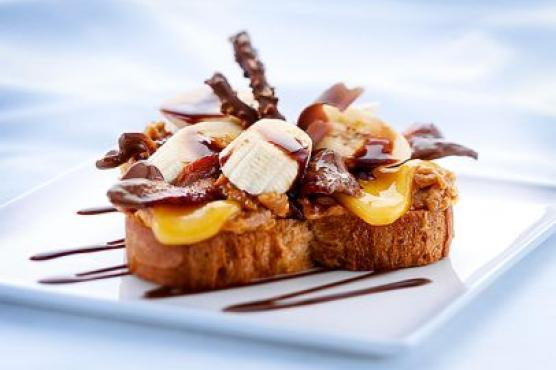
\includegraphics[width=\linewidth]{images/evaluation-images/grilled_cheese_sandwich/grilled-cheese-sandwich457.jpeg}
\end{minipage}
\hfill
\begin{minipage}[t]{0.5\textwidth}
	\vspace{0pt}\raggedright
	\begin{tabularx}{\textwidth}{X r}
		\small \textbf{Real class} & \small Grilled Cheese Sandwich\\
		\small \textbf{Predicted class} & \small Muffin\\
		\small \textbf{Predicted accuracy} & \small 61.15 \%
    \end{tabularx}\\
    
    \vspace{6pt}
	\begin{tabularx}{\textwidth}{X r}
        \small \textbf{Top-5} & \small \textbf{Accuracy} \\
        \hline
		\small 1) Muffin & \small 61.15 \%\\\small 2) Cinnamon Roll & \small 11.50 \%\\\small 3) Waffles & \small 10.79 \%\\\small 4) Cheesecake & \small 7.04 \%\\\small 5) Kebabs & \small 3.11 \%
    \end{tabularx}
\end{minipage}
    
\subsection{Ice Cream}
    
\subsubsection{ice\textunderscore cream/ice-cream70.jpg}

\begin{minipage}[t]{0.4\textwidth}
	\vspace{0pt}
	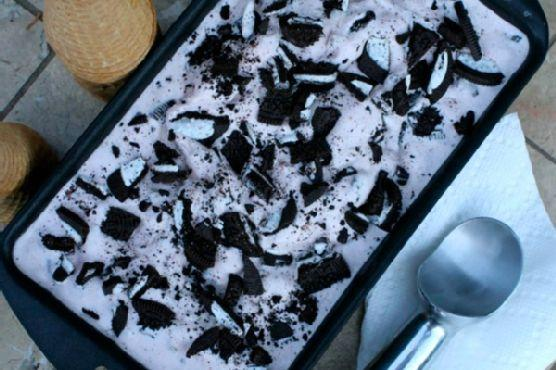
\includegraphics[width=\linewidth]{images/evaluation-images/ice_cream/ice-cream70.jpg}
\end{minipage}
\hfill
\begin{minipage}[t]{0.5\textwidth}
	\vspace{0pt}\raggedright
	\begin{tabularx}{\textwidth}{X r}
		\small \textbf{Real class} & \small Ice Cream\\
		\small \textbf{Predicted class} & \small Brownies\\
		\small \textbf{Predicted accuracy} & \small 93.38 \%
    \end{tabularx}\\
    
    \vspace{6pt}
	\begin{tabularx}{\textwidth}{X r}
        \small \textbf{Top-5} & \small \textbf{Accuracy} \\
        \hline
		\small 1) Brownies & \small 93.38 \%\\\small 2) Cheesecake & \small 2.09 \%\\\small 3) Lasagne & \small 1.02 \%\\\small 4) Smoothie & \small 0.75 \%\\\small 5) Mashed Potatoes & \small 0.56 \%
    \end{tabularx}
\end{minipage}
    
\subsection{Kebabs}
    
\subsubsection{kebabs/kebabs208.png}

\begin{minipage}[t]{0.4\textwidth}
	\vspace{0pt}
	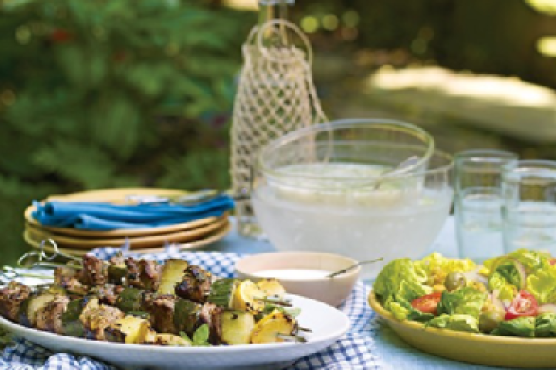
\includegraphics[width=\linewidth]{images/evaluation-images/kebabs/kebabs208.png}
\end{minipage}
\hfill
\begin{minipage}[t]{0.5\textwidth}
	\vspace{0pt}\raggedright
	\begin{tabularx}{\textwidth}{X r}
		\small \textbf{Real class} & \small Kebabs\\
		\small \textbf{Predicted class} & \small Salad\\
		\small \textbf{Predicted accuracy} & \small 99.52 \%
    \end{tabularx}\\
    
    \vspace{6pt}
	\begin{tabularx}{\textwidth}{X r}
        \small \textbf{Top-5} & \small \textbf{Accuracy} \\
        \hline
		\small 1) Salad & \small 99.52 \%\\\small 2) Caesar Salad & \small 0.23 \%\\\small 3) Guacamole & \small 0.21 \%\\\small 4) Cobb Salad & \small 0.02 \%\\\small 5) Margarita & \small 0.01 \%
    \end{tabularx}
\end{minipage}
    
\subsubsection{kebabs/kebabs212.jpg}

\begin{minipage}[t]{0.4\textwidth}
	\vspace{0pt}
	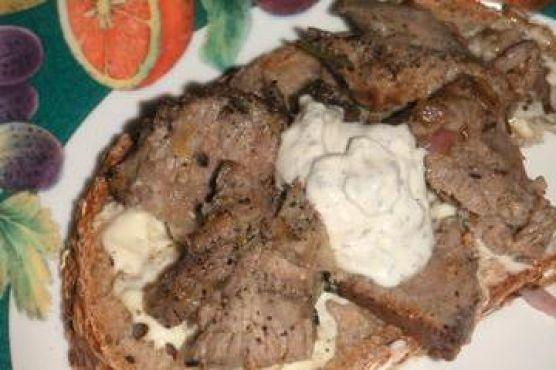
\includegraphics[width=\linewidth]{images/evaluation-images/kebabs/kebabs212.jpg}
\end{minipage}
\hfill
\begin{minipage}[t]{0.5\textwidth}
	\vspace{0pt}\raggedright
	\begin{tabularx}{\textwidth}{X r}
		\small \textbf{Real class} & \small Kebabs\\
		\small \textbf{Predicted class} & \small Beef Stew\\
		\small \textbf{Predicted accuracy} & \small 69.13 \%
    \end{tabularx}\\
    
    \vspace{6pt}
	\begin{tabularx}{\textwidth}{X r}
        \small \textbf{Top-5} & \small \textbf{Accuracy} \\
        \hline
		\small 1) Beef Stew & \small 69.13 \%\\\small 2) Brownies & \small 16.67 \%\\\small 3) Meatballs & \small 5.50 \%\\\small 4) Beef Stroganoff & \small 2.45 \%\\\small 5) Meatloaf & \small 2.02 \%
    \end{tabularx}
\end{minipage}
    
\subsubsection{kebabs/kebabs218.jpg}

\begin{minipage}[t]{0.4\textwidth}
	\vspace{0pt}
	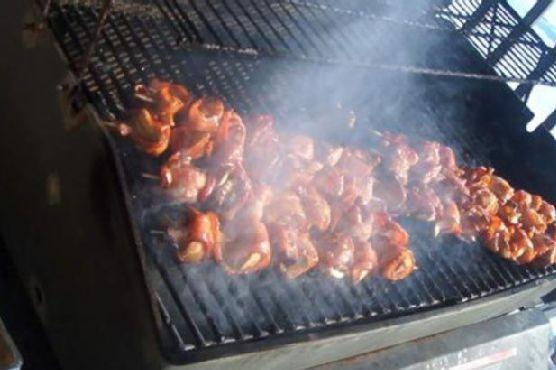
\includegraphics[width=\linewidth]{images/evaluation-images/kebabs/kebabs218.jpg}
\end{minipage}
\hfill
\begin{minipage}[t]{0.5\textwidth}
	\vspace{0pt}\raggedright
	\begin{tabularx}{\textwidth}{X r}
		\small \textbf{Real class} & \small Kebabs\\
		\small \textbf{Predicted class} & \small Cheesecake\\
		\small \textbf{Predicted accuracy} & \small 40.02 \%
    \end{tabularx}\\
    
    \vspace{6pt}
	\begin{tabularx}{\textwidth}{X r}
        \small \textbf{Top-5} & \small \textbf{Accuracy} \\
        \hline
		\small 1) Cheesecake & \small 40.02 \%\\\small 2) Baked Beans & \small 25.64 \%\\\small 3) Brownies & \small 17.66 \%\\\small 4) Bundt Cake & \small 3.99 \%\\\small 5) Muffin & \small 3.19 \%
    \end{tabularx}
\end{minipage}
    
\subsubsection{kebabs/kebabs229.jpg}

\begin{minipage}[t]{0.4\textwidth}
	\vspace{0pt}
	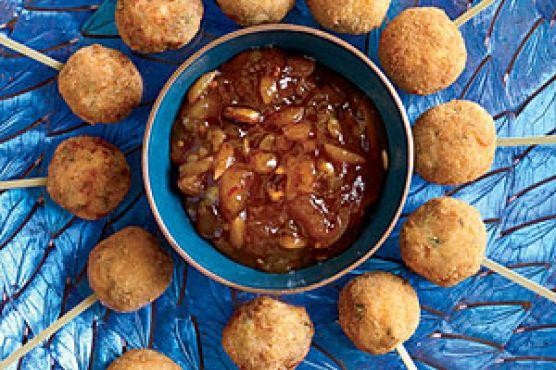
\includegraphics[width=\linewidth]{images/evaluation-images/kebabs/kebabs229.jpg}
\end{minipage}
\hfill
\begin{minipage}[t]{0.5\textwidth}
	\vspace{0pt}\raggedright
	\begin{tabularx}{\textwidth}{X r}
		\small \textbf{Real class} & \small Kebabs\\
		\small \textbf{Predicted class} & \small Muffin\\
		\small \textbf{Predicted accuracy} & \small 98.20 \%
    \end{tabularx}\\
    
    \vspace{6pt}
	\begin{tabularx}{\textwidth}{X r}
        \small \textbf{Top-5} & \small \textbf{Accuracy} \\
        \hline
		\small 1) Muffin & \small 98.20 \%\\\small 2) Meatballs & \small 1.24 \%\\\small 3) Baked Beans & \small 0.50 \%\\\small 4) Corn Dog & \small 0.04 \%\\\small 5) Soup & \small 0.00 \%
    \end{tabularx}
\end{minipage}
    
\subsubsection{kebabs/kebabs54.jpg}

\begin{minipage}[t]{0.4\textwidth}
	\vspace{0pt}
	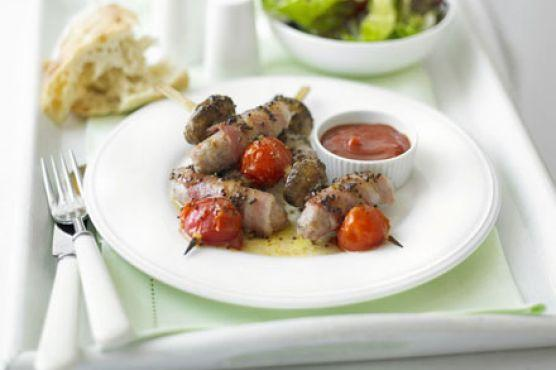
\includegraphics[width=\linewidth]{images/evaluation-images/kebabs/kebabs54.jpg}
\end{minipage}
\hfill
\begin{minipage}[t]{0.5\textwidth}
	\vspace{0pt}\raggedright
	\begin{tabularx}{\textwidth}{X r}
		\small \textbf{Real class} & \small Kebabs\\
		\small \textbf{Predicted class} & \small Omelet\\
		\small \textbf{Predicted accuracy} & \small 42.18 \%
    \end{tabularx}\\
    
    \vspace{6pt}
	\begin{tabularx}{\textwidth}{X r}
        \small \textbf{Top-5} & \small \textbf{Accuracy} \\
        \hline
		\small 1) Omelet & \small 42.18 \%\\\small 2) Beef Stew & \small 27.91 \%\\\small 3) Soup & \small 11.56 \%\\\small 4) Frittata & \small 5.67 \%\\\small 5) Salad & \small 5.08 \%
    \end{tabularx}
\end{minipage}
    
\subsubsection{kebabs/kebabs7.jpg}

\begin{minipage}[t]{0.4\textwidth}
	\vspace{0pt}
	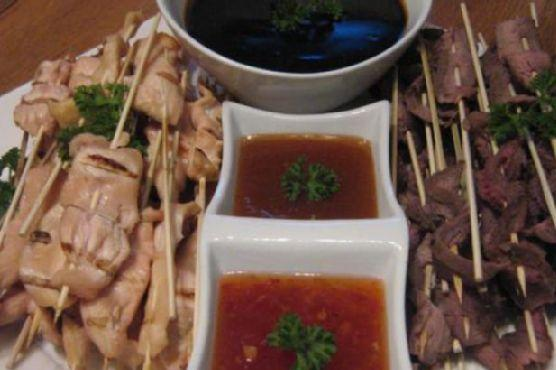
\includegraphics[width=\linewidth]{images/evaluation-images/kebabs/kebabs7.jpg}
\end{minipage}
\hfill
\begin{minipage}[t]{0.5\textwidth}
	\vspace{0pt}\raggedright
	\begin{tabularx}{\textwidth}{X r}
		\small \textbf{Real class} & \small Kebabs\\
		\small \textbf{Predicted class} & \small Meatballs\\
		\small \textbf{Predicted accuracy} & \small 22.81 \%
    \end{tabularx}\\
    
    \vspace{6pt}
	\begin{tabularx}{\textwidth}{X r}
        \small \textbf{Top-5} & \small \textbf{Accuracy} \\
        \hline
		\small 1) Meatballs & \small 22.81 \%\\\small 2) Soup & \small 16.27 \%\\\small 3) Beef Stew & \small 14.27 \%\\\small 4) Coleslaw & \small 11.13 \%\\\small 5) Cheesecake & \small 7.48 \%
    \end{tabularx}
\end{minipage}
    
\subsection{Key Lime Pie}
    
\subsubsection{key\textunderscore lime\textunderscore pie/key-lime-pie66.jpg}

\begin{minipage}[t]{0.4\textwidth}
	\vspace{0pt}
	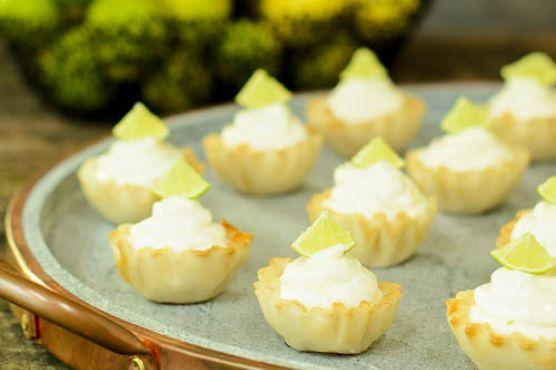
\includegraphics[width=\linewidth]{images/evaluation-images/key_lime_pie/key-lime-pie66.jpg}
\end{minipage}
\hfill
\begin{minipage}[t]{0.5\textwidth}
	\vspace{0pt}\raggedright
	\begin{tabularx}{\textwidth}{X r}
		\small \textbf{Real class} & \small Key Lime Pie\\
		\small \textbf{Predicted class} & \small Muffin\\
		\small \textbf{Predicted accuracy} & \small 56.63 \%
    \end{tabularx}\\
    
    \vspace{6pt}
	\begin{tabularx}{\textwidth}{X r}
        \small \textbf{Top-5} & \small \textbf{Accuracy} \\
        \hline
		\small 1) Muffin & \small 56.63 \%\\\small 2) Stuffed Pepper & \small 37.31 \%\\\small 3) Donut & \small 3.18 \%\\\small 4) Cheesecake & \small 1.47 \%\\\small 5) Popcorn & \small 0.58 \%
    \end{tabularx}
\end{minipage}
    
\subsection{Lasagne}
    
\subsubsection{lasagne/lasagne165.png}

\begin{minipage}[t]{0.4\textwidth}
	\vspace{0pt}
	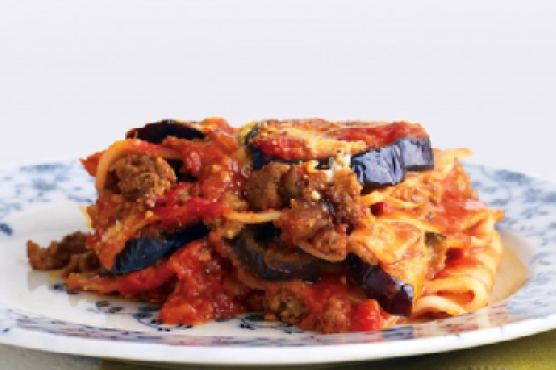
\includegraphics[width=\linewidth]{images/evaluation-images/lasagne/lasagne165.png}
\end{minipage}
\hfill
\begin{minipage}[t]{0.5\textwidth}
	\vspace{0pt}\raggedright
	\begin{tabularx}{\textwidth}{X r}
		\small \textbf{Real class} & \small Lasagne\\
		\small \textbf{Predicted class} & \small Nachos\\
		\small \textbf{Predicted accuracy} & \small 83.50 \%
    \end{tabularx}\\
    
    \vspace{6pt}
	\begin{tabularx}{\textwidth}{X r}
        \small \textbf{Top-5} & \small \textbf{Accuracy} \\
        \hline
		\small 1) Nachos & \small 83.50 \%\\\small 2) Kebabs & \small 14.12 \%\\\small 3) Quesadilla & \small 1.38 \%\\\small 4) Meatballs & \small 0.26 \%\\\small 5) Frittata & \small 0.20 \%
    \end{tabularx}
\end{minipage}
    
\subsubsection{lasagne/lasagne310.jpg}

\begin{minipage}[t]{0.4\textwidth}
	\vspace{0pt}
	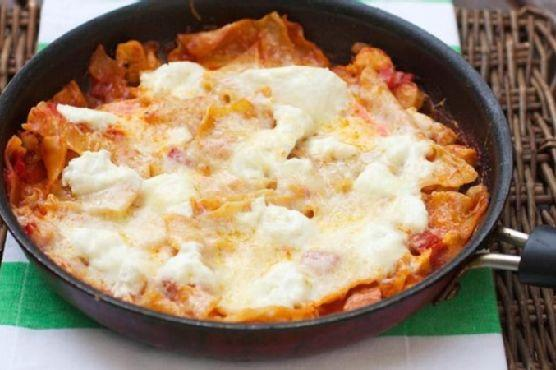
\includegraphics[width=\linewidth]{images/evaluation-images/lasagne/lasagne310.jpg}
\end{minipage}
\hfill
\begin{minipage}[t]{0.5\textwidth}
	\vspace{0pt}\raggedright
	\begin{tabularx}{\textwidth}{X r}
		\small \textbf{Real class} & \small Lasagne\\
		\small \textbf{Predicted class} & \small Frittata\\
		\small \textbf{Predicted accuracy} & \small 99.57 \%
    \end{tabularx}\\
    
    \vspace{6pt}
	\begin{tabularx}{\textwidth}{X r}
        \small \textbf{Top-5} & \small \textbf{Accuracy} \\
        \hline
		\small 1) Frittata & \small 99.57 \%\\\small 2) Mashed Potatoes & \small 0.31 \%\\\small 3) Beef Stew & \small 0.03 \%\\\small 4) Coleslaw & \small 0.02 \%\\\small 5) Soup & \small 0.01 \%
    \end{tabularx}
\end{minipage}
    
\subsubsection{lasagne/lasagne443.jpeg}

\begin{minipage}[t]{0.4\textwidth}
	\vspace{0pt}
	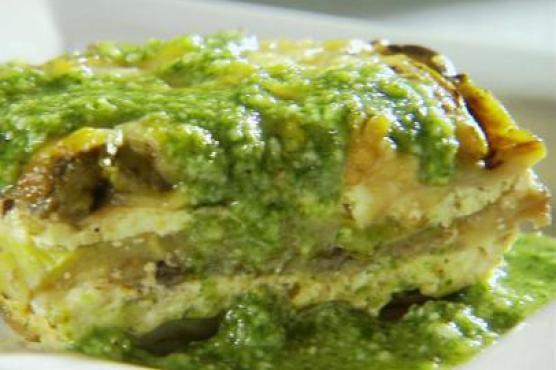
\includegraphics[width=\linewidth]{images/evaluation-images/lasagne/lasagne443.jpeg}
\end{minipage}
\hfill
\begin{minipage}[t]{0.5\textwidth}
	\vspace{0pt}\raggedright
	\begin{tabularx}{\textwidth}{X r}
		\small \textbf{Real class} & \small Lasagne\\
		\small \textbf{Predicted class} & \small Guacamole\\
		\small \textbf{Predicted accuracy} & \small 97.45 \%
    \end{tabularx}\\
    
    \vspace{6pt}
	\begin{tabularx}{\textwidth}{X r}
        \small \textbf{Top-5} & \small \textbf{Accuracy} \\
        \hline
		\small 1) Guacamole & \small 97.45 \%\\\small 2) Mashed Potatoes & \small 0.98 \%\\\small 3) Frittata & \small 0.57 \%\\\small 4) Creamed Spinach & \small 0.19 \%\\\small 5) Soup & \small 0.18 \%
    \end{tabularx}
\end{minipage}
    
\subsubsection{lasagne/lasagne449.jpeg}

\begin{minipage}[t]{0.4\textwidth}
	\vspace{0pt}
	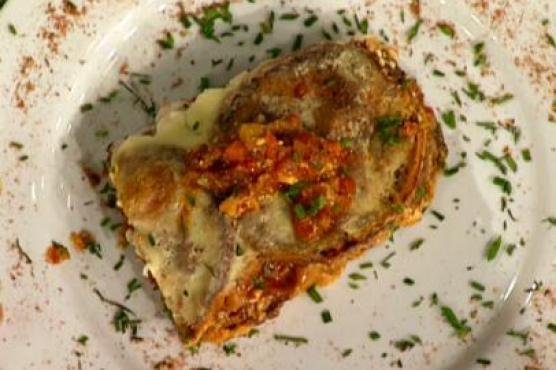
\includegraphics[width=\linewidth]{images/evaluation-images/lasagne/lasagne449.jpeg}
\end{minipage}
\hfill
\begin{minipage}[t]{0.5\textwidth}
	\vspace{0pt}\raggedright
	\begin{tabularx}{\textwidth}{X r}
		\small \textbf{Real class} & \small Lasagne\\
		\small \textbf{Predicted class} & \small Frittata\\
		\small \textbf{Predicted accuracy} & \small 33.95 \%
    \end{tabularx}\\
    
    \vspace{6pt}
	\begin{tabularx}{\textwidth}{X r}
        \small \textbf{Top-5} & \small \textbf{Accuracy} \\
        \hline
		\small 1) Frittata & \small 33.95 \%\\\small 2) Grilled Cheese Sandwich & \small 17.48 \%\\\small 3) Omelet & \small 15.73 \%\\\small 4) Bundt Cake & \small 8.82 \%\\\small 5) Baked Salmon & \small 8.44 \%
    \end{tabularx}
\end{minipage}
    
\subsection{Macaroni And Cheese}
    
\subsubsection{macaroni\textunderscore and\textunderscore cheese/macaroni-and-cheese186.jpg}

\begin{minipage}[t]{0.4\textwidth}
	\vspace{0pt}
	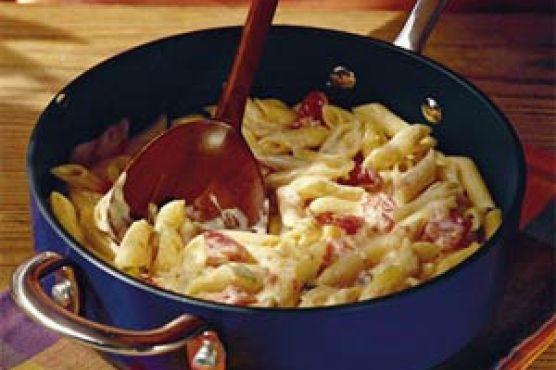
\includegraphics[width=\linewidth]{images/evaluation-images/macaroni_and_cheese/macaroni-and-cheese186.jpg}
\end{minipage}
\hfill
\begin{minipage}[t]{0.5\textwidth}
	\vspace{0pt}\raggedright
	\begin{tabularx}{\textwidth}{X r}
		\small \textbf{Real class} & \small Macaroni And Cheese\\
		\small \textbf{Predicted class} & \small Coleslaw\\
		\small \textbf{Predicted accuracy} & \small 90.56 \%
    \end{tabularx}\\
    
    \vspace{6pt}
	\begin{tabularx}{\textwidth}{X r}
        \small \textbf{Top-5} & \small \textbf{Accuracy} \\
        \hline
		\small 1) Coleslaw & \small 90.56 \%\\\small 2) Beef Stew & \small 6.28 \%\\\small 3) Soup & \small 1.06 \%\\\small 4) Spaghetti & \small 0.56 \%\\\small 5) Frittata & \small 0.37 \%
    \end{tabularx}
\end{minipage}
    
\subsubsection{macaroni\textunderscore and\textunderscore cheese/macaroni-and-cheese432.jpeg}

\begin{minipage}[t]{0.4\textwidth}
	\vspace{0pt}
	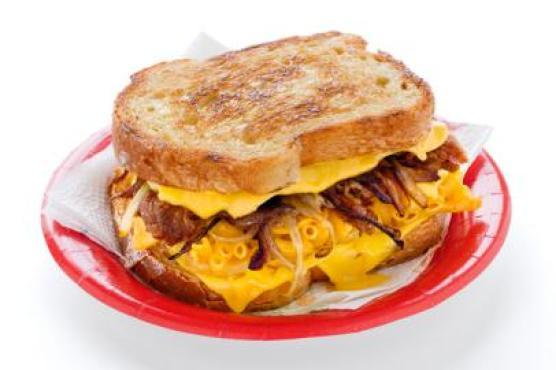
\includegraphics[width=\linewidth]{images/evaluation-images/macaroni_and_cheese/macaroni-and-cheese432.jpeg}
\end{minipage}
\hfill
\begin{minipage}[t]{0.5\textwidth}
	\vspace{0pt}\raggedright
	\begin{tabularx}{\textwidth}{X r}
		\small \textbf{Real class} & \small Macaroni And Cheese\\
		\small \textbf{Predicted class} & \small Grilled Cheese Sandwich\\
		\small \textbf{Predicted accuracy} & \small 99.90 \%
    \end{tabularx}\\
    
    \vspace{6pt}
	\begin{tabularx}{\textwidth}{X r}
        \small \textbf{Top-5} & \small \textbf{Accuracy} \\
        \hline
		\small 1) Grilled Cheese Sandwich & \small 99.90 \%\\\small 2) Burger & \small 0.09 \%\\\small 3) Lasagne & \small 0.00 \%\\\small 4) Quesadilla & \small 0.00 \%\\\small 5) Waffles & \small 0.00 \%
    \end{tabularx}
\end{minipage}
    
\subsection{Meatballs}
    
\subsubsection{meatballs/meatballs14.jpg}

\begin{minipage}[t]{0.4\textwidth}
	\vspace{0pt}
	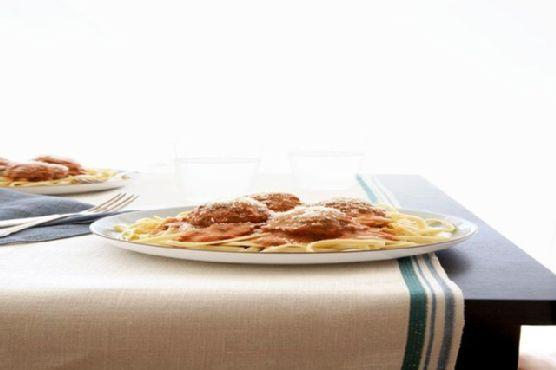
\includegraphics[width=\linewidth]{images/evaluation-images/meatballs/meatballs14.jpg}
\end{minipage}
\hfill
\begin{minipage}[t]{0.5\textwidth}
	\vspace{0pt}\raggedright
	\begin{tabularx}{\textwidth}{X r}
		\small \textbf{Real class} & \small Meatballs\\
		\small \textbf{Predicted class} & \small Pancakes\\
		\small \textbf{Predicted accuracy} & \small 67.29 \%
    \end{tabularx}\\
    
    \vspace{6pt}
	\begin{tabularx}{\textwidth}{X r}
        \small \textbf{Top-5} & \small \textbf{Accuracy} \\
        \hline
		\small 1) Pancakes & \small 67.29 \%\\\small 2) Waffles & \small 17.07 \%\\\small 3) Empanada & \small 3.77 \%\\\small 4) Cheesecake & \small 3.24 \%\\\small 5) Quesadilla & \small 1.65 \%
    \end{tabularx}
\end{minipage}
    
\subsubsection{meatballs/meatballs298.jpg}

\begin{minipage}[t]{0.4\textwidth}
	\vspace{0pt}
	\includegraphics[width=\linewidth]{images/evaluation-images/meatballs/meatballs298.jpg}
\end{minipage}
\hfill
\begin{minipage}[t]{0.5\textwidth}
	\vspace{0pt}\raggedright
	\begin{tabularx}{\textwidth}{X r}
		\small \textbf{Real class} & \small Meatballs\\
		\small \textbf{Predicted class} & \small Pancakes\\
		\small \textbf{Predicted accuracy} & \small 99.82 \%
    \end{tabularx}\\
    
    \vspace{6pt}
	\begin{tabularx}{\textwidth}{X r}
        \small \textbf{Top-5} & \small \textbf{Accuracy} \\
        \hline
		\small 1) Pancakes & \small 99.82 \%\\\small 2) Burger & \small 0.05 \%\\\small 3) Cheesecake & \small 0.03 \%\\\small 4) Margarita & \small 0.02 \%\\\small 5) Grilled Cheese Sandwich & \small 0.02 \%
    \end{tabularx}
\end{minipage}
    
\subsubsection{meatballs/meatballs59.png}

\begin{minipage}[t]{0.4\textwidth}
	\vspace{0pt}
	\includegraphics[width=\linewidth]{images/evaluation-images/meatballs/meatballs59.png}
\end{minipage}
\hfill
\begin{minipage}[t]{0.5\textwidth}
	\vspace{0pt}\raggedright
	\begin{tabularx}{\textwidth}{X r}
		\small \textbf{Real class} & \small Meatballs\\
		\small \textbf{Predicted class} & \small Cinnamon Roll\\
		\small \textbf{Predicted accuracy} & \small 92.34 \%
    \end{tabularx}\\
    
    \vspace{6pt}
	\begin{tabularx}{\textwidth}{X r}
        \small \textbf{Top-5} & \small \textbf{Accuracy} \\
        \hline
		\small 1) Cinnamon Roll & \small 92.34 \%\\\small 2) Donut & \small 7.44 \%\\\small 3) Corn Dog & \small 0.04 \%\\\small 4) Beef Stroganoff & \small 0.03 \%\\\small 5) Kebabs & \small 0.03 \%
    \end{tabularx}
\end{minipage}
    
\subsection{Meatloaf}
    
\subsubsection{meatloaf/meatloaf151.jpg}

\begin{minipage}[t]{0.4\textwidth}
	\vspace{0pt}
	\includegraphics[width=\linewidth]{images/evaluation-images/meatloaf/meatloaf151.jpg}
\end{minipage}
\hfill
\begin{minipage}[t]{0.5\textwidth}
	\vspace{0pt}\raggedright
	\begin{tabularx}{\textwidth}{X r}
		\small \textbf{Real class} & \small Meatloaf\\
		\small \textbf{Predicted class} & \small Chicken Wings\\
		\small \textbf{Predicted accuracy} & \small 57.50 \%
    \end{tabularx}\\
    
    \vspace{6pt}
	\begin{tabularx}{\textwidth}{X r}
        \small \textbf{Top-5} & \small \textbf{Accuracy} \\
        \hline
		\small 1) Chicken Wings & \small 57.50 \%\\\small 2) Soup & \small 31.97 \%\\\small 3) Beef Stew & \small 5.16 \%\\\small 4) Meatballs & \small 1.43 \%\\\small 5) Lasagne & \small 0.92 \%
    \end{tabularx}
\end{minipage}
    
\subsubsection{meatloaf/meatloaf152.jpg}

\begin{minipage}[t]{0.4\textwidth}
	\vspace{0pt}
	\includegraphics[width=\linewidth]{images/evaluation-images/meatloaf/meatloaf152.jpg}
\end{minipage}
\hfill
\begin{minipage}[t]{0.5\textwidth}
	\vspace{0pt}\raggedright
	\begin{tabularx}{\textwidth}{X r}
		\small \textbf{Real class} & \small Meatloaf\\
		\small \textbf{Predicted class} & \small Nachos\\
		\small \textbf{Predicted accuracy} & \small 96.56 \%
    \end{tabularx}\\
    
    \vspace{6pt}
	\begin{tabularx}{\textwidth}{X r}
        \small \textbf{Top-5} & \small \textbf{Accuracy} \\
        \hline
		\small 1) Nachos & \small 96.56 \%\\\small 2) Waffles & \small 1.81 \%\\\small 3) Cinnamon Roll & \small 0.69 \%\\\small 4) Beef Stroganoff & \small 0.28 \%\\\small 5) Lasagne & \small 0.20 \%
    \end{tabularx}
\end{minipage}
    
\subsubsection{meatloaf/meatloaf351.jpg}

\begin{minipage}[t]{0.4\textwidth}
	\vspace{0pt}
	\includegraphics[width=\linewidth]{images/evaluation-images/meatloaf/meatloaf351.jpg}
\end{minipage}
\hfill
\begin{minipage}[t]{0.5\textwidth}
	\vspace{0pt}\raggedright
	\begin{tabularx}{\textwidth}{X r}
		\small \textbf{Real class} & \small Meatloaf\\
		\small \textbf{Predicted class} & \small Pancakes\\
		\small \textbf{Predicted accuracy} & \small 80.10 \%
    \end{tabularx}\\
    
    \vspace{6pt}
	\begin{tabularx}{\textwidth}{X r}
        \small \textbf{Top-5} & \small \textbf{Accuracy} \\
        \hline
		\small 1) Pancakes & \small 80.10 \%\\\small 2) Bundt Cake & \small 4.85 \%\\\small 3) Quesadilla & \small 2.82 \%\\\small 4) Grilled Cheese Sandwich & \small 2.63 \%\\\small 5) Cinnamon Roll & \small 1.89 \%
    \end{tabularx}
\end{minipage}
    
\subsubsection{meatloaf/meatloaf367.jpeg}

\begin{minipage}[t]{0.4\textwidth}
	\vspace{0pt}
	\includegraphics[width=\linewidth]{images/evaluation-images/meatloaf/meatloaf367.jpeg}
\end{minipage}
\hfill
\begin{minipage}[t]{0.5\textwidth}
	\vspace{0pt}\raggedright
	\begin{tabularx}{\textwidth}{X r}
		\small \textbf{Real class} & \small Meatloaf\\
		\small \textbf{Predicted class} & \small Muffin\\
		\small \textbf{Predicted accuracy} & \small 99.45 \%
    \end{tabularx}\\
    
    \vspace{6pt}
	\begin{tabularx}{\textwidth}{X r}
        \small \textbf{Top-5} & \small \textbf{Accuracy} \\
        \hline
		\small 1) Muffin & \small 99.45 \%\\\small 2) Frittata & \small 0.34 \%\\\small 3) Lasagne & \small 0.12 \%\\\small 4) Meatballs & \small 0.03 \%\\\small 5) Brownies & \small 0.03 \%
    \end{tabularx}
\end{minipage}
    
\subsubsection{meatloaf/meatloaf427.jpeg}

\begin{minipage}[t]{0.4\textwidth}
	\vspace{0pt}
	\includegraphics[width=\linewidth]{images/evaluation-images/meatloaf/meatloaf427.jpeg}
\end{minipage}
\hfill
\begin{minipage}[t]{0.5\textwidth}
	\vspace{0pt}\raggedright
	\begin{tabularx}{\textwidth}{X r}
		\small \textbf{Real class} & \small Meatloaf\\
		\small \textbf{Predicted class} & \small Pancakes\\
		\small \textbf{Predicted accuracy} & \small 40.19 \%
    \end{tabularx}\\
    
    \vspace{6pt}
	\begin{tabularx}{\textwidth}{X r}
        \small \textbf{Top-5} & \small \textbf{Accuracy} \\
        \hline
		\small 1) Pancakes & \small 40.19 \%\\\small 2) Burger & \small 23.83 \%\\\small 3) Grilled Cheese Sandwich & \small 9.87 \%\\\small 4) Cheesecake & \small 8.19 \%\\\small 5) Omelet & \small 5.15 \%
    \end{tabularx}
\end{minipage}
    
\subsection{Muffin}
    
\subsubsection{muffin/muffin131.jpg}

\begin{minipage}[t]{0.4\textwidth}
	\vspace{0pt}
	\includegraphics[width=\linewidth]{images/evaluation-images/muffin/muffin131.jpg}
\end{minipage}
\hfill
\begin{minipage}[t]{0.5\textwidth}
	\vspace{0pt}\raggedright
	\begin{tabularx}{\textwidth}{X r}
		\small \textbf{Real class} & \small Muffin\\
		\small \textbf{Predicted class} & \small Cheesecake\\
		\small \textbf{Predicted accuracy} & \small 54.46 \%
    \end{tabularx}\\
    
    \vspace{6pt}
	\begin{tabularx}{\textwidth}{X r}
        \small \textbf{Top-5} & \small \textbf{Accuracy} \\
        \hline
		\small 1) Cheesecake & \small 54.46 \%\\\small 2) Bundt Cake & \small 35.09 \%\\\small 3) Grilled Cheese Sandwich & \small 9.87 \%\\\small 4) Brownies & \small 0.18 \%\\\small 5) Donut & \small 0.13 \%
    \end{tabularx}
\end{minipage}
    
\subsection{Nachos}
    
\subsubsection{nachos/nachos202.jpg}

\begin{minipage}[t]{0.4\textwidth}
	\vspace{0pt}
	\includegraphics[width=\linewidth]{images/evaluation-images/nachos/nachos202.jpg}
\end{minipage}
\hfill
\begin{minipage}[t]{0.5\textwidth}
	\vspace{0pt}\raggedright
	\begin{tabularx}{\textwidth}{X r}
		\small \textbf{Real class} & \small Nachos\\
		\small \textbf{Predicted class} & \small Salad\\
		\small \textbf{Predicted accuracy} & \small 57.92 \%
    \end{tabularx}\\
    
    \vspace{6pt}
	\begin{tabularx}{\textwidth}{X r}
        \small \textbf{Top-5} & \small \textbf{Accuracy} \\
        \hline
		\small 1) Salad & \small 57.92 \%\\\small 2) Popcorn & \small 13.09 \%\\\small 3) Chicken Wings & \small 12.50 \%\\\small 4) Lasagne & \small 3.74 \%\\\small 5) Meatballs & \small 3.70 \%
    \end{tabularx}
\end{minipage}
    
\subsubsection{nachos/nachos98.jpg}

\begin{minipage}[t]{0.4\textwidth}
	\vspace{0pt}
	\includegraphics[width=\linewidth]{images/evaluation-images/nachos/nachos98.jpg}
\end{minipage}
\hfill
\begin{minipage}[t]{0.5\textwidth}
	\vspace{0pt}\raggedright
	\begin{tabularx}{\textwidth}{X r}
		\small \textbf{Real class} & \small Nachos\\
		\small \textbf{Predicted class} & \small Frittata\\
		\small \textbf{Predicted accuracy} & \small 99.75 \%
    \end{tabularx}\\
    
    \vspace{6pt}
	\begin{tabularx}{\textwidth}{X r}
        \small \textbf{Top-5} & \small \textbf{Accuracy} \\
        \hline
		\small 1) Frittata & \small 99.75 \%\\\small 2) Omelet & \small 0.08 \%\\\small 3) Mashed Potatoes & \small 0.04 \%\\\small 4) Beef Stew & \small 0.03 \%\\\small 5) Pancakes & \small 0.02 \%
    \end{tabularx}
\end{minipage}
    
\subsection{Omelet}
    
\subsubsection{omelet/omelet138.jpg}

\begin{minipage}[t]{0.4\textwidth}
	\vspace{0pt}
	\includegraphics[width=\linewidth]{images/evaluation-images/omelet/omelet138.jpg}
\end{minipage}
\hfill
\begin{minipage}[t]{0.5\textwidth}
	\vspace{0pt}\raggedright
	\begin{tabularx}{\textwidth}{X r}
		\small \textbf{Real class} & \small Omelet\\
		\small \textbf{Predicted class} & \small Pancakes\\
		\small \textbf{Predicted accuracy} & \small 78.32 \%
    \end{tabularx}\\
    
    \vspace{6pt}
	\begin{tabularx}{\textwidth}{X r}
        \small \textbf{Top-5} & \small \textbf{Accuracy} \\
        \hline
		\small 1) Pancakes & \small 78.32 \%\\\small 2) Beef Stew & \small 12.49 \%\\\small 3) Chicken Wings & \small 4.68 \%\\\small 4) Waffles & \small 1.12 \%\\\small 5) Cheesecake & \small 0.40 \%
    \end{tabularx}
\end{minipage}
    
\subsubsection{omelet/omelet397.jpg}

\begin{minipage}[t]{0.4\textwidth}
	\vspace{0pt}
	\includegraphics[width=\linewidth]{images/evaluation-images/omelet/omelet397.jpg}
\end{minipage}
\hfill
\begin{minipage}[t]{0.5\textwidth}
	\vspace{0pt}\raggedright
	\begin{tabularx}{\textwidth}{X r}
		\small \textbf{Real class} & \small Omelet\\
		\small \textbf{Predicted class} & \small Pancakes\\
		\small \textbf{Predicted accuracy} & \small 49.17 \%
    \end{tabularx}\\
    
    \vspace{6pt}
	\begin{tabularx}{\textwidth}{X r}
        \small \textbf{Top-5} & \small \textbf{Accuracy} \\
        \hline
		\small 1) Pancakes & \small 49.17 \%\\\small 2) Pizza & \small 36.92 \%\\\small 3) Chicken Piccata & \small 9.34 \%\\\small 4) Quesadilla & \small 2.54 \%\\\small 5) Buttermilk Biscuits & \small 0.33 \%
    \end{tabularx}
\end{minipage}
    
\subsubsection{omelet/omelet403.jpg}

\begin{minipage}[t]{0.4\textwidth}
	\vspace{0pt}
	\includegraphics[width=\linewidth]{images/evaluation-images/omelet/omelet403.jpg}
\end{minipage}
\hfill
\begin{minipage}[t]{0.5\textwidth}
	\vspace{0pt}\raggedright
	\begin{tabularx}{\textwidth}{X r}
		\small \textbf{Real class} & \small Omelet\\
		\small \textbf{Predicted class} & \small Nachos\\
		\small \textbf{Predicted accuracy} & \small 50.77 \%
    \end{tabularx}\\
    
    \vspace{6pt}
	\begin{tabularx}{\textwidth}{X r}
        \small \textbf{Top-5} & \small \textbf{Accuracy} \\
        \hline
		\small 1) Nachos & \small 50.77 \%\\\small 2) Pizza & \small 16.93 \%\\\small 3) Frittata & \small 15.08 \%\\\small 4) Beef Stew & \small 2.71 \%\\\small 5) Lasagne & \small 2.63 \%
    \end{tabularx}
\end{minipage}
    
\subsubsection{omelet/omelet56.jpg}

\begin{minipage}[t]{0.4\textwidth}
	\vspace{0pt}
	\includegraphics[width=\linewidth]{images/evaluation-images/omelet/omelet56.jpg}
\end{minipage}
\hfill
\begin{minipage}[t]{0.5\textwidth}
	\vspace{0pt}\raggedright
	\begin{tabularx}{\textwidth}{X r}
		\small \textbf{Real class} & \small Omelet\\
		\small \textbf{Predicted class} & \small Guacamole\\
		\small \textbf{Predicted accuracy} & \small 64.24 \%
    \end{tabularx}\\
    
    \vspace{6pt}
	\begin{tabularx}{\textwidth}{X r}
        \small \textbf{Top-5} & \small \textbf{Accuracy} \\
        \hline
		\small 1) Guacamole & \small 64.24 \%\\\small 2) Burrito & \small 29.77 \%\\\small 3) Quesadilla & \small 3.03 \%\\\small 4) Nachos & \small 0.63 \%\\\small 5) Frittata & \small 0.55 \%
    \end{tabularx}
\end{minipage}
    
\subsection{Pancakes}
    
\subsubsection{pancakes/pancakes357.jpg}

\begin{minipage}[t]{0.4\textwidth}
	\vspace{0pt}
	\includegraphics[width=\linewidth]{images/evaluation-images/pancakes/pancakes357.jpg}
\end{minipage}
\hfill
\begin{minipage}[t]{0.5\textwidth}
	\vspace{0pt}\raggedright
	\begin{tabularx}{\textwidth}{X r}
		\small \textbf{Real class} & \small Pancakes\\
		\small \textbf{Predicted class} & \small Brownies\\
		\small \textbf{Predicted accuracy} & \small 35.50 \%
    \end{tabularx}\\
    
    \vspace{6pt}
	\begin{tabularx}{\textwidth}{X r}
        \small \textbf{Top-5} & \small \textbf{Accuracy} \\
        \hline
		\small 1) Brownies & \small 35.50 \%\\\small 2) Popcorn & \small 26.05 \%\\\small 3) Frittata & \small 9.03 \%\\\small 4) Cheesecake & \small 9.02 \%\\\small 5) Muffin & \small 7.34 \%
    \end{tabularx}
\end{minipage}
    
\subsection{Pizza}
    
\subsubsection{pizza/pizza116.jpg}

\begin{minipage}[t]{0.4\textwidth}
	\vspace{0pt}
	\includegraphics[width=\linewidth]{images/evaluation-images/pizza/pizza116.jpg}
\end{minipage}
\hfill
\begin{minipage}[t]{0.5\textwidth}
	\vspace{0pt}\raggedright
	\begin{tabularx}{\textwidth}{X r}
		\small \textbf{Real class} & \small Pizza\\
		\small \textbf{Predicted class} & \small Calzone\\
		\small \textbf{Predicted accuracy} & \small 98.48 \%
    \end{tabularx}\\
    
    \vspace{6pt}
	\begin{tabularx}{\textwidth}{X r}
        \small \textbf{Top-5} & \small \textbf{Accuracy} \\
        \hline
		\small 1) Calzone & \small 98.48 \%\\\small 2) Empanada & \small 1.42 \%\\\small 3) Quesadilla & \small 0.04 \%\\\small 4) Muffin & \small 0.01 \%\\\small 5) Omelet & \small 0.01 \%
    \end{tabularx}
\end{minipage}
    
\subsection{Quesadilla}
    
\subsubsection{quesadilla/quesadilla230.jpg}

\begin{minipage}[t]{0.4\textwidth}
	\vspace{0pt}
	\includegraphics[width=\linewidth]{images/evaluation-images/quesadilla/quesadilla230.jpg}
\end{minipage}
\hfill
\begin{minipage}[t]{0.5\textwidth}
	\vspace{0pt}\raggedright
	\begin{tabularx}{\textwidth}{X r}
		\small \textbf{Real class} & \small Quesadilla\\
		\small \textbf{Predicted class} & \small Omelet\\
		\small \textbf{Predicted accuracy} & \small 45.38 \%
    \end{tabularx}\\
    
    \vspace{6pt}
	\begin{tabularx}{\textwidth}{X r}
        \small \textbf{Top-5} & \small \textbf{Accuracy} \\
        \hline
		\small 1) Omelet & \small 45.38 \%\\\small 2) Lasagne & \small 14.68 \%\\\small 3) Corn Dog & \small 12.58 \%\\\small 4) Mashed Potatoes & \small 9.45 \%\\\small 5) Baked Salmon & \small 5.27 \%
    \end{tabularx}
\end{minipage}
    
\subsubsection{quesadilla/quesadilla281.jpg}

\begin{minipage}[t]{0.4\textwidth}
	\vspace{0pt}
	\includegraphics[width=\linewidth]{images/evaluation-images/quesadilla/quesadilla281.jpg}
\end{minipage}
\hfill
\begin{minipage}[t]{0.5\textwidth}
	\vspace{0pt}\raggedright
	\begin{tabularx}{\textwidth}{X r}
		\small \textbf{Real class} & \small Quesadilla\\
		\small \textbf{Predicted class} & \small Cinnamon Roll\\
		\small \textbf{Predicted accuracy} & \small 99.74 \%
    \end{tabularx}\\
    
    \vspace{6pt}
	\begin{tabularx}{\textwidth}{X r}
        \small \textbf{Top-5} & \small \textbf{Accuracy} \\
        \hline
		\small 1) Cinnamon Roll & \small 99.74 \%\\\small 2) Donut & \small 0.17 \%\\\small 3) Pancakes & \small 0.05 \%\\\small 4) Pizza & \small 0.01 \%\\\small 5) Bundt Cake & \small 0.01 \%
    \end{tabularx}
\end{minipage}
    
\subsection{Salad}
    
\subsubsection{salad/salad482.jpg}

\begin{minipage}[t]{0.4\textwidth}
	\vspace{0pt}
	\includegraphics[width=\linewidth]{images/evaluation-images/salad/salad482.jpg}
\end{minipage}
\hfill
\begin{minipage}[t]{0.5\textwidth}
	\vspace{0pt}\raggedright
	\begin{tabularx}{\textwidth}{X r}
		\small \textbf{Real class} & \small Salad\\
		\small \textbf{Predicted class} & \small Spaghetti\\
		\small \textbf{Predicted accuracy} & \small 97.68 \%
    \end{tabularx}\\
    
    \vspace{6pt}
	\begin{tabularx}{\textwidth}{X r}
        \small \textbf{Top-5} & \small \textbf{Accuracy} \\
        \hline
		\small 1) Spaghetti & \small 97.68 \%\\\small 2) Omelet & \small 0.63 \%\\\small 3) Macaroni And Cheese & \small 0.36 \%\\\small 4) French Fries & \small 0.32 \%\\\small 5) Coleslaw & \small 0.25 \%
    \end{tabularx}
\end{minipage}
    
\subsubsection{salad/salad67.jpg}

\begin{minipage}[t]{0.4\textwidth}
	\vspace{0pt}
	\includegraphics[width=\linewidth]{images/evaluation-images/salad/salad67.jpg}
\end{minipage}
\hfill
\begin{minipage}[t]{0.5\textwidth}
	\vspace{0pt}\raggedright
	\begin{tabularx}{\textwidth}{X r}
		\small \textbf{Real class} & \small Salad\\
		\small \textbf{Predicted class} & \small Popcorn\\
		\small \textbf{Predicted accuracy} & \small 52.37 \%
    \end{tabularx}\\
    
    \vspace{6pt}
	\begin{tabularx}{\textwidth}{X r}
        \small \textbf{Top-5} & \small \textbf{Accuracy} \\
        \hline
		\small 1) Popcorn & \small 52.37 \%\\\small 2) Nachos & \small 36.51 \%\\\small 3) Macaroni And Cheese & \small 4.29 \%\\\small 4) Pizza & \small 1.87 \%\\\small 5) Mashed Potatoes & \small 1.72 \%
    \end{tabularx}
\end{minipage}
    
\subsection{Soup}
    
\subsubsection{soup/soup146.jpg}

\begin{minipage}[t]{0.4\textwidth}
	\vspace{0pt}
	\includegraphics[width=\linewidth]{images/evaluation-images/soup/soup146.jpg}
\end{minipage}
\hfill
\begin{minipage}[t]{0.5\textwidth}
	\vspace{0pt}\raggedright
	\begin{tabularx}{\textwidth}{X r}
		\small \textbf{Real class} & \small Soup\\
		\small \textbf{Predicted class} & \small Baked Beans\\
		\small \textbf{Predicted accuracy} & \small 78.82 \%
    \end{tabularx}\\
    
    \vspace{6pt}
	\begin{tabularx}{\textwidth}{X r}
        \small \textbf{Top-5} & \small \textbf{Accuracy} \\
        \hline
		\small 1) Baked Beans & \small 78.82 \%\\\small 2) Chicken Wings & \small 6.64 \%\\\small 3) Meatballs & \small 6.54 \%\\\small 4) Popcorn & \small 6.03 \%\\\small 5) Beef Stew & \small 0.86 \%
    \end{tabularx}
\end{minipage}
    
\subsubsection{soup/soup23.jpg}

\begin{minipage}[t]{0.4\textwidth}
	\vspace{0pt}
	\includegraphics[width=\linewidth]{images/evaluation-images/soup/soup23.jpg}
\end{minipage}
\hfill
\begin{minipage}[t]{0.5\textwidth}
	\vspace{0pt}\raggedright
	\begin{tabularx}{\textwidth}{X r}
		\small \textbf{Real class} & \small Soup\\
		\small \textbf{Predicted class} & \small Salad\\
		\small \textbf{Predicted accuracy} & \small 50.30 \%
    \end{tabularx}\\
    
    \vspace{6pt}
	\begin{tabularx}{\textwidth}{X r}
        \small \textbf{Top-5} & \small \textbf{Accuracy} \\
        \hline
		\small 1) Salad & \small 50.30 \%\\\small 2) Baked Beans & \small 17.44 \%\\\small 3) Pizza & \small 10.81 \%\\\small 4) Lasagne & \small 3.97 \%\\\small 5) Burrito & \small 3.50 \%
    \end{tabularx}
\end{minipage}
    
\subsubsection{soup/soup247.jpg}

\begin{minipage}[t]{0.4\textwidth}
	\vspace{0pt}
	\includegraphics[width=\linewidth]{images/evaluation-images/soup/soup247.jpg}
\end{minipage}
\hfill
\begin{minipage}[t]{0.5\textwidth}
	\vspace{0pt}\raggedright
	\begin{tabularx}{\textwidth}{X r}
		\small \textbf{Real class} & \small Soup\\
		\small \textbf{Predicted class} & \small Cobb Salad\\
		\small \textbf{Predicted accuracy} & \small 99.67 \%
    \end{tabularx}\\
    
    \vspace{6pt}
	\begin{tabularx}{\textwidth}{X r}
        \small \textbf{Top-5} & \small \textbf{Accuracy} \\
        \hline
		\small 1) Cobb Salad & \small 99.67 \%\\\small 2) Salad & \small 0.13 \%\\\small 3) Coleslaw & \small 0.13 \%\\\small 4) Baked Salmon & \small 0.02 \%\\\small 5) Spaghetti & \small 0.02 \%
    \end{tabularx}
\end{minipage}
    
\subsubsection{soup/soup414.jpg}

\begin{minipage}[t]{0.4\textwidth}
	\vspace{0pt}
	\includegraphics[width=\linewidth]{images/evaluation-images/soup/soup414.jpg}
\end{minipage}
\hfill
\begin{minipage}[t]{0.5\textwidth}
	\vspace{0pt}\raggedright
	\begin{tabularx}{\textwidth}{X r}
		\small \textbf{Real class} & \small Soup\\
		\small \textbf{Predicted class} & \small Burrito\\
		\small \textbf{Predicted accuracy} & \small 24.99 \%
    \end{tabularx}\\
    
    \vspace{6pt}
	\begin{tabularx}{\textwidth}{X r}
        \small \textbf{Top-5} & \small \textbf{Accuracy} \\
        \hline
		\small 1) Burrito & \small 24.99 \%\\\small 2) Omelet & \small 23.75 \%\\\small 3) Quesadilla & \small 21.07 \%\\\small 4) Guacamole & \small 19.41 \%\\\small 5) Nachos & \small 6.83 \%
    \end{tabularx}
\end{minipage}
    
\subsection{Stuffed Pepper}
    
\subsubsection{stuffed\textunderscore pepper/stuffed-pepper118.jpg}

\begin{minipage}[t]{0.4\textwidth}
	\vspace{0pt}
	\includegraphics[width=\linewidth]{images/evaluation-images/stuffed_pepper/stuffed-pepper118.jpg}
\end{minipage}
\hfill
\begin{minipage}[t]{0.5\textwidth}
	\vspace{0pt}\raggedright
	\begin{tabularx}{\textwidth}{X r}
		\small \textbf{Real class} & \small Stuffed Pepper\\
		\small \textbf{Predicted class} & \small Meatballs\\
		\small \textbf{Predicted accuracy} & \small 90.61 \%
    \end{tabularx}\\
    
    \vspace{6pt}
	\begin{tabularx}{\textwidth}{X r}
        \small \textbf{Top-5} & \small \textbf{Accuracy} \\
        \hline
		\small 1) Meatballs & \small 90.61 \%\\\small 2) Meatloaf & \small 1.96 \%\\\small 3) Baked Salmon & \small 1.72 \%\\\small 4) Kebabs & \small 1.47 \%\\\small 5) Spaghetti & \small 0.75 \%
    \end{tabularx}
\end{minipage}
    
\subsection{Waffles}
    
\subsubsection{waffles/waffles155.png}

\begin{minipage}[t]{0.4\textwidth}
	\vspace{0pt}
	\includegraphics[width=\linewidth]{images/evaluation-images/waffles/waffles155.png}
\end{minipage}
\hfill
\begin{minipage}[t]{0.5\textwidth}
	\vspace{0pt}\raggedright
	\begin{tabularx}{\textwidth}{X r}
		\small \textbf{Real class} & \small Waffles\\
		\small \textbf{Predicted class} & \small Meatloaf\\
		\small \textbf{Predicted accuracy} & \small 85.85 \%
    \end{tabularx}\\
    
    \vspace{6pt}
	\begin{tabularx}{\textwidth}{X r}
        \small \textbf{Top-5} & \small \textbf{Accuracy} \\
        \hline
		\small 1) Meatloaf & \small 85.85 \%\\\small 2) Cinnamon Roll & \small 3.61 \%\\\small 3) Burger & \small 3.39 \%\\\small 4) Grilled Cheese Sandwich & \small 2.94 \%\\\small 5) Chicken Wings & \small 1.75 \%
    \end{tabularx}
\end{minipage}
    
\subsubsection{waffles/waffles470.jpg}

\begin{minipage}[t]{0.4\textwidth}
	\vspace{0pt}
	\includegraphics[width=\linewidth]{images/evaluation-images/waffles/waffles470.jpg}
\end{minipage}
\hfill
\begin{minipage}[t]{0.5\textwidth}
	\vspace{0pt}\raggedright
	\begin{tabularx}{\textwidth}{X r}
		\small \textbf{Real class} & \small Waffles\\
		\small \textbf{Predicted class} & \small Pizza\\
		\small \textbf{Predicted accuracy} & \small 97.55 \%
    \end{tabularx}\\
    
    \vspace{6pt}
	\begin{tabularx}{\textwidth}{X r}
        \small \textbf{Top-5} & \small \textbf{Accuracy} \\
        \hline
		\small 1) Pizza & \small 97.55 \%\\\small 2) Cheesecake & \small 1.18 \%\\\small 3) Donut & \small 0.84 \%\\\small 4) Pancakes & \small 0.16 \%\\\small 5) Burger & \small 0.07 \%
    \end{tabularx}
\end{minipage}
    
\subsubsection{waffles/waffles487.jpg}

\begin{minipage}[t]{0.4\textwidth}
	\vspace{0pt}
	\includegraphics[width=\linewidth]{images/evaluation-images/waffles/waffles487.jpg}
\end{minipage}
\hfill
\begin{minipage}[t]{0.5\textwidth}
	\vspace{0pt}\raggedright
	\begin{tabularx}{\textwidth}{X r}
		\small \textbf{Real class} & \small Waffles\\
		\small \textbf{Predicted class} & \small Meatballs\\
		\small \textbf{Predicted accuracy} & \small 39.50 \%
    \end{tabularx}\\
    
    \vspace{6pt}
	\begin{tabularx}{\textwidth}{X r}
        \small \textbf{Top-5} & \small \textbf{Accuracy} \\
        \hline
		\small 1) Meatballs & \small 39.50 \%\\\small 2) Beef Stroganoff & \small 37.33 \%\\\small 3) Burger & \small 12.47 \%\\\small 4) Nachos & \small 3.91 \%\\\small 5) Calzone & \small 2.66 \%
    \end{tabularx}
\end{minipage}
    
	\pagebreak

\end{document}